\chapter{Реализация клиентской части информационной системы «Личный кабинет абитуриента»}

Клиентская часть информационной системы «Личный кабинет абитуриента» будет реализована на базе JavaScript фреймворка Vue.js. Архитектура веб-приложения реализована при помощи Model-View-Controller паттерна, позволяя разделить клиентское приложение на модель, представление и контроллер, благодаря чему модификация одного из этих компонентов оказывает минимальное воздействие на остальные или не оказывает его вовсе \cite{mvcpattern}.

Стартовой точкой веб-приложения является файл \verb|main.js|, в нем подключаются все используемые библиотеки, а также в функцию \verb|createApp| передается базовый компонент, используемый во всем приложении \cite{vuemainjs}.

Для создания контроллера использована официальная библиотека маршрутизации для Vue.js — Vue Router. Контроллер отвечает за навигацию внутри клиентского приложения и обработку пользовательских событий.

В объявленном массиве маршрутов, каждый маршрут содержит название, путь, компонент, который будет отображен при переходе по маршруту (листинг \ref{ls:router}). В мета данных содержится уровень доступа к маршруту и шаблон, в который будет вставлен отображаемый компонент \cite{vuejsrouter}.

\begin{lstlisting}[caption={Примеры объявленных маршрутов}, label={ls:router}]
{
  path: '/submit-consent/:id',
  name: 'SubmitConsentView',
  component: () => import(/* webpackChunkName: "submit-consent" */ '../views/SubmitConsentView.vue'),
  meta: {
    privilege: 20,
    layout: 'DashboardLayout',
  },
},
{
  path: '/statement/:id',
  name: 'StatementView',
  component: () => import(/* webpackChunkName: "statement-id" */ '../views/StatementView.vue'),
  meta: {
    privilege: 20,
    layout: 'DashboardLayout',
  },
},
\end{lstlisting}

В шаблон базового компонента \verb|App.vue| вставлен компонент \verb|AppLayout.vue|, в слот которого передается компонент, указанный в маршруте. \verb|AppLayout.vue| реализует подключение шаблона, указанного в мета данных маршрута, а в случае его отсутствие подключает шаблон по умолчанию (листинг \ref{ls:applayout}) \cite{vuelayout}. Пример того, как взаимосвязаны компоненты, при открытии страницы подачи заявления, можно увидеть на диаграмме компонентов (рисунок \ref{fig:diagramcomponent}).

\begin{lstlisting}[caption={Реализация компонента AppLayout}, label={ls:applayout}]
<template>
  <div>
    <keep-alive>
      <component :is="layout">
        <slot/>
      </component>
    </keep-alive>
  </div>
</template>

<script>
import { ref, watch, markRaw } from 'vue';
import { useRoute } from 'vue-router';

export default {
  name: 'AppLayout',
  setup() {
    const route = useRoute();
    const layout = ref();
    const getLayout = async (lyt) => {
      const c = await import(`@/layouts/${lyt}.vue`);
      return c.default;
    };
    watch(
      () => route.meta,
      async (meta) => {
        try {
          layout.value = markRaw(await getLayout(meta.layout));
        } catch (e) {
          console.warn('%c Use AppLayoutDefault instead.\n', 'color: darkturquoise', e);
          layout.value = markRaw(await getLayout('DefaultLayout'));
        }
      }
    );
    return { layout };
  },
};
</script>
\end{lstlisting}

\begin{figure}[H]
\begin{center}
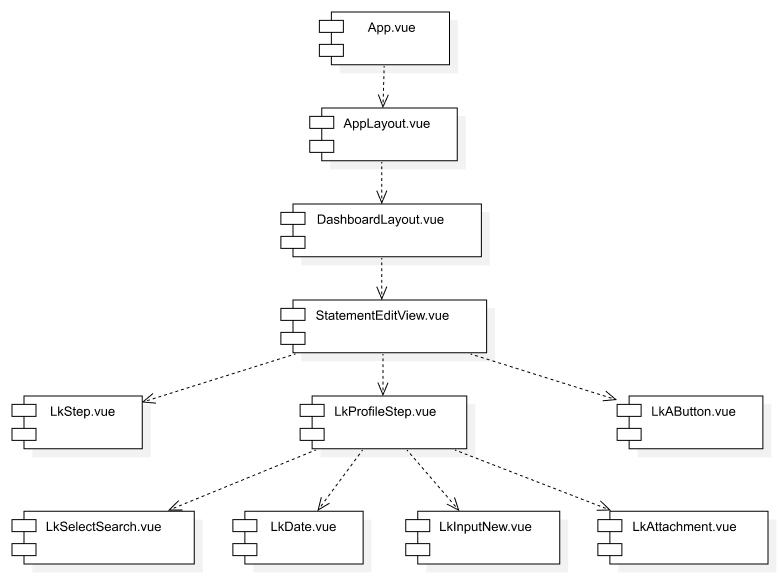
\includegraphics[width=0.9\hsize]{fig/diagram-components.png}\\[2mm]
\caption{Диаграмма компонентов}\label{fig:diagramcomponent}
\end{center}
\end{figure}

Модель отвечает за хранение и работку с данными. Для реализации модели используется официальная библиотека для Vue.js — Vuex. Она служит централизованным хранилищем данных для всех компонентов приложения с правилами, гарантирующими, что состояние может быть изменено только предсказуемым образом. Единственный способ внести изменения в состояние данных — вызвать мутацию. Для удобства, взаимодействие с API сервисов вынесено в отдельные файлы \cite{vuex}.

Так, модуль аутентификации содержит в качестве состояния объект user, в котором содержатся поля loggedIn, status, token. Действия используют методы сервисов, которые выполняют запросы к API, после чего вызывают мутации, которые в свою очередь выполняют изменения состояния хранилища (листинг \ref{ls:vuex}).

\begin{lstlisting}[caption={Реализация действия авторизации}, label={ls:vuex}]
    login({ commit }, user) {
      return AuthService.login(user).then(
        // eslint-disable-next-line no-shadow
        (user) => {
          commit('loginSuccess', user);
          return Promise.resolve(user);
        },
        (error) => {
          console.log('Login false!');
          console.log(error);
          commit('loginFailure');
          return Promise.reject(error);
        },
      );
    },
\end{lstlisting}

\section{Реализация процесса аутентификации пользователя}

Процесс проверки подлинности пользователя реализован с помощью технологии JSON Web Token (JWT). JWT — это открытый стандарт (RFC 7519) для создания токенов доступа, основанный на формате JSON. Токены выпускаются сервером аутентификации, подписываются с помощью секретного ключа и передаются клиенту, который в дальнейшем использует данный токен для аутентификации при выполнении запросов к серверу.

Сервер выпускает новые токены при прохождении авторизации и подтверждении новой учетной записи, созданные токены записываются и хранятся в локальном хранилище в браузере пользователя. При каждом запросе к API, заголовок, содержащий JWT, добавляется к запросу, для этого реализована функция \verb|authHeader|, которая создает заголовок аутентификации, используя в качестве значения токен, хранящийся в локальном хранилище (листинг \ref{ls:headerauth}) \cite{jwt}.

\begin{lstlisting}[caption={Реализация функции создающей заголовок аутентификации}, label={ls:headerauth}]
export default function authHeader(file = false) {
  const token = JSON.parse(localStorage.getItem('token'));

  if (token) {
    return {
      ContentType: file === false ? 'application/json' :  'multipart/form-data',
      Authorization: `Bearer ${token}`
    };
  }
  return {};
}
\end{lstlisting}

\section{Реализация взаимодействия с пользовательским вводом}

Для реализации удобного взаимодействия с веб-приложением, на формах (листинг \ref{ls:fieldexp}) используется валидации ввода в режиме реального времени (листинг \ref{ls:fieldvalidation}), таким образом, пользователь получает информацию об ошибках до момента отправки формы на сервер (рисунок \ref{fig:regvalidation}). Так же на формах используются маски ввода, которые подсказывают формат определенных полей, таких как СНИЛС, номер телефона, и т.п.

\begin{lstlisting}[caption={Пример реализации поля в шаблоне}, label={ls:fieldexp}]
<div class="reg__input">
  <div class="reg__input__title require">E-mail</div>
  <lk-input-new v-model:value="v$.form.email.value.$model" @blur="v$.form.email.value.$touch" placeHolder="Введите e-mail" height="48px"></lk-input-new>
  <div v-for="error of v$.form.email.value.$errors" :key="error.$uid">
    <div class="input_error">{{ error.$message }}</div>
  </div>
  <div v-for="error of form.email.errors" :key="error">
    <div class="input_error">{{ error }}</div>
  </div>
</div>
\end{lstlisting}

\begin{lstlisting}[caption={Пример определения правил валидации поля}, label={ls:fieldvalidation}]
email: {
  value: {
    required: helpers.withMessage('Поле не заполнено', required),
      email: helpers.withMessage('Введен некорректный e-mail', email),
      $lazy: true,
      $autoDirty: true,
  },
},
\end{lstlisting}

\begin{figure}[H]
\begin{center}
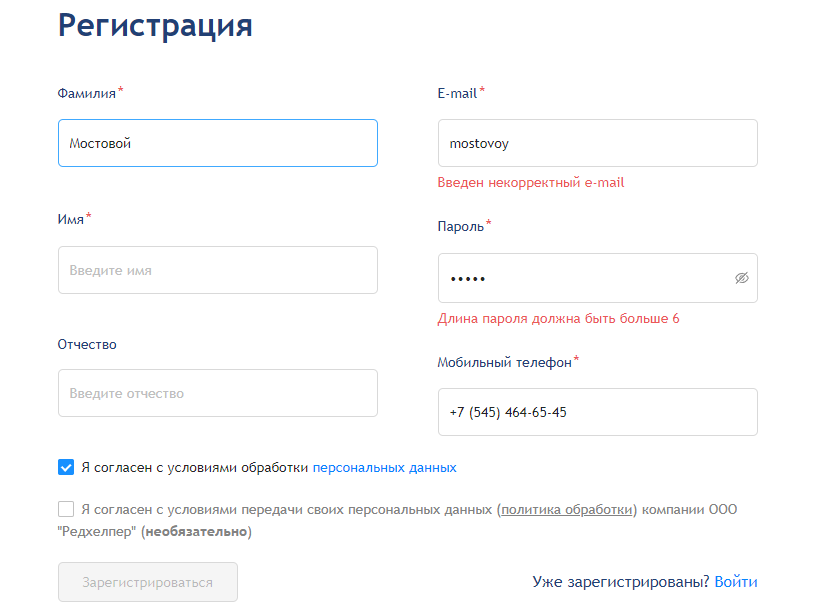
\includegraphics[width=0.9\hsize]{fig/reg.png}\\[2mm]
\caption{Пример валидации полей формы}\label{fig:regvalidation}
\end{center}
\end{figure}

На внутренних страницах личного кабинета, реализована отправка формы после окончания взаимодействия с любым полем (листинг \ref{ls:fieldlkemp}) (рисунок \ref{fig:inputsave}), все поля формы, которые изменялись пользователем за время работы с приложением проходят валидацию (листинг \ref{ls:fieldlksaving}), после чего отправляются на сервер, таким образом, пустые поля, которые не затрагивались пользователем не вызовут сообщение об ошибке.

\begin{lstlisting}[caption={Пример поля с отправкой данных на сервер после окончания взаимодействия}, label={ls:fieldlkemp}]
<div class="input">
  <div class="input__text">
    <div class="input__title require">Дата рождения</div>
    <div :class="{ input__status__disable: form.dob.saved }" class="input__status">Сохранено</div>
</div>
  <lk-date
    v-model="v$.form.dob.value.$model"
    backgroundColor="transparent"
    placeHolder="Выберите дату рождения"
    @blur="v$.form.dob.value.$touch"
    @change="savingData('dob')"
    @focus="form.dob.saved = false"
    ></lk-date>

  <div v-for="error of v$.form.dob.value.$errors" :key="error.$uid">
    <div class="input_error">{{ error.$message }}</div>
  </div>

  <div v-for="error of form.dob.errors" :key="error">
    <div class="input_error">{{ error }}</div>
  </div>
</div>
\end{lstlisting}

\begin{lstlisting}[caption={Метод валидирующий поле и передающий данные для отправки на сервер}, label={ls:fieldlksaving}]
savingData(key, validate = true) {
  if (validate) {
    this.v$.form[key].value.$touch();

    if (this.v$.form[key].value.$error) {
      this.form[key].saved = false;
      return;
    }
  }

  this.setUserProfile(key);
  this.form[key].saved = true;
},
\end{lstlisting}

\begin{figure}[H]
\begin{center}
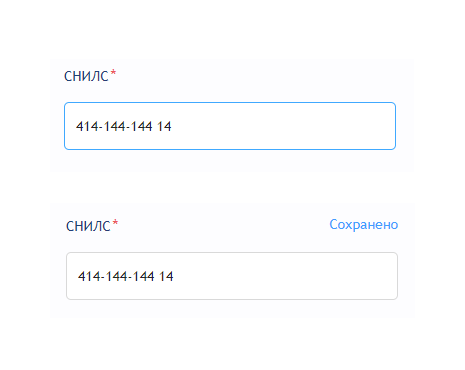
\includegraphics[width=0.6\hsize]{fig/input-save.png}\\[2mm]
\caption{Пример сохранения данных после окончания взаимодействия с полем}\label{fig:inputsave}
\end{center}
\end{figure}

\section{Реализация процесса регистрации пользователя}

Для регистрации учетной записи необходимо заполнить форму регистрации, после чего на указанный в форме e-mail адрес будет отправлено письмо для подтверждения учетной записи. В письме содержится сгенерированная ссылка (пример сгенерированной ссылки: https://abit.lk.volsu.ru/confirm-email/activate/61d7369014662), при переходе по ней осуществляется подтверждение учетной записи (рисунок \ref{fig:confirmemail}).

\begin{figure}[H]
\begin{center}

\includegraphics[width=0.8\hsize]{fig/confirm-email.png}\\[2mm]
\caption{Письмо для подтверждения учетной записи}\label{fig:confirmemail}
\end{center}
\end{figure}

При переходе по ссылке, контроллер (листинг \ref{ls:activateroute}) отображает компонент \verb|ConfirmEmailActivateView.vue|, в котором происходит подтверждение учетной записи. Уникальный код активации, содержащийся в ссылке, передается в действие глобального хранилище (листинг \ref{ls:activatecomponent}), после чего отправляется на сервер, в случае успешной активации, сервер возвращает JWT, статус учетной записи и уровень доступа, вызванные внутри действия мутации меняют состояние приложения (листинг \ref{ls:vuexactivate}), записывают в локальное хранилище уровень доступа и JWT, после чего пользователь перенаправляется на внутреннюю страницу личного кабинета.

\begin{lstlisting}[caption={Маршрут активации учетной записи}, label={ls:activateroute}]
{
  path: '/confirm-email/:email', 
  name: 'ConfirmEmailView',
  component: () => import(/* webpackChunkName: "confirm-email" */ '../views/ConfirmEmailView.vue'),
  meta: {
    layout: 'AuthLayout',
  },
},
\end{lstlisting}

\begin{lstlisting}[caption={Реализация компонента активации учетной записи}, label={ls:activatecomponent}]
mounted() {
  const user = new FormData();
  user.append('code', this.$route.params.activate);

  this.$store.dispatch('auth/activate', user).then(
    () => {
      this.message = 'Email confirm!';
      this.$router.push('/');
    },
    error => {
      console.log(error);
      // eslint-disable-next-line no-unused-vars
      Object.entries(error).forEach(([key, value]) =>
        // eslint-disable-next-line no-return-assign
        error[key].forEach(i =>
          this.message = i
        )
      )
    }
  );
},
\end{lstlisting}

\begin{lstlisting}[caption={Реализация действия в глобальном хранилище, активирующее учетную запись}, label={ls:vuexactivate}]
activate({ commit }, user) {
  return AuthService.activate(user).then(
    // eslint-disable-next-line no-shadow
    (user) => {
      commit('activateSuccess', user);
      return Promise.resolve(user);
    },
    (error) => {
      console.log('Activate false!');
      console.log(error);
      commit('activateFailure');
      return Promise.reject(error);
    },
  );
},
\end{lstlisting}

\section{Реализация процесса авторизации пользователя}

Для прохождения авторизации, пользователь должен заполнить форму, состоящую из e-mail адреса и пароля. Введенные данные передаются в действие глобального хранилище (листинг \ref{ls:singinmethod}), после чего отправляется на сервер, в случае успешной авторизации, сервер возвращает JWT, статус учетной записи и уровень доступа (рисунок \ref{fig:singinserverresponse}), вызванные внутри действия мутации меняют состояние приложения (листинг \ref{ls:vuexlogin}), записывают в локальное хранилище уровень доступа и JWT, после чего пользователь перенаправляется на внутреннюю страницу личного кабинета.

\begin{lstlisting}[caption={Метод передающий форму в действие глобального хранилища}, label={ls:singinmethod}]
singIn() {
  const user = new FormData();
  // eslint-disable-next-line no-unused-vars
  Object.entries(this.form).forEach(([key, value]) => user.append(key, this.form[key].value));
  this.$store.dispatch('auth/login', user).then(
    () => {
      this.$router.push('/');
    },
    error => {
      // eslint-disable-next-line no-unused-vars
      Object.entries(error).forEach(([key, value]) => {
        this.form[key].errors = []
        error[key].forEach(i => this.form[key].errors.push(i));
      });
    }
  );
},
\end{lstlisting}

\begin{lstlisting}[caption={Реализация действия в глобальном хранилище, активирующее авторизацию}, label={ls:vuexlogin}]
login({ commit }, user) {
  return AuthService.login(user).then(
    // eslint-disable-next-line no-shadow
    (user) => {
      commit('loginSuccess', user);
      return Promise.resolve(user);
    },
    (error) => {
      console.log('Login false!');
      console.log(error);
      commit('loginFailure');
      return Promise.reject(error);
    },
  );
},
\end{lstlisting}

\begin{figure}[H]
\begin{center}
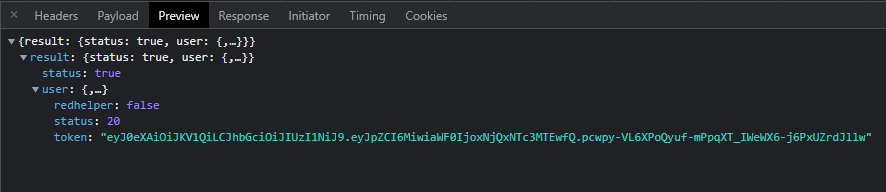
\includegraphics[width=0.9\hsize]{fig/login-server-response.png}\\[2mm]
\caption{Ответ сервера на успешный запрос авторизации}\label{fig:singinserverresponse}
\end{center}
\end{figure}

В случае, если пользователь не помнит пароль от учетной записи, на странице восстановления пароля, он должен указать e-mail адрес учетной записи, куда придет письмо c ссылкой для восстановления пароля (рисунок \ref{fig:recoverypass}). При переходе по ссылке, пользователь должен указать новый пароль для учетной записи (рисунок \ref{fig:recoverypassform}), после чего будет перенаправлен на страницу авторизации.

\begin{figure}[H]
\begin{center}

\includegraphics[width=0.9\hsize]{fig/recovery-pass.png}\\[2mm]
\caption{Писмо для восстановления пароля от учетной записи}\label{fig:recoverypass}
\end{center}
\end{figure}

\begin{figure}[H]
\begin{center}

\includegraphics[width=0.9\hsize]{fig/recovery-pass-form.png}\\[2mm]
\caption{Форма восстановления пароля от учетной записи}\label{fig:recoverypassform}
\end{center}
\end{figure}

\section{Реализация процесса подачи заявления на поступление}

Процесс подачи заявления разбит на семь этапов, на каждом из которых абитуриент вводит информацию, необходимую для подачи заявления, которая будет использована для автоматической генерации бланка подачи заявления.

Этапы «профиль» и «персональные данные» являются общими для всех уровней образования, т.е при редактировании данных на этих этапах на любом из уровней образования, изменения произойдут сразу на всех уровнях.

Этапы могут заполняться в произвольном порядке, а благодаря сохранению данных при окончании взаимодействия с любым полем, продолжить заполнять заявление можно на любом устройстве.

\subsection{Реализация этапа заполнения профиля абитуриента}

На данном этапе, пользователь заполняет основную информацию о себе. Данные указанные при регистрации, а именно имя, фамилия, отчество, телефон, и электронная почта будут автоматически пред заполнены (рисунок \ref{fig:profilestep}). Поле электронной почты является неизменяемым, поскольку оно является идентифицирующем для учетной записи.

\begin{figure}[H]
\begin{center}
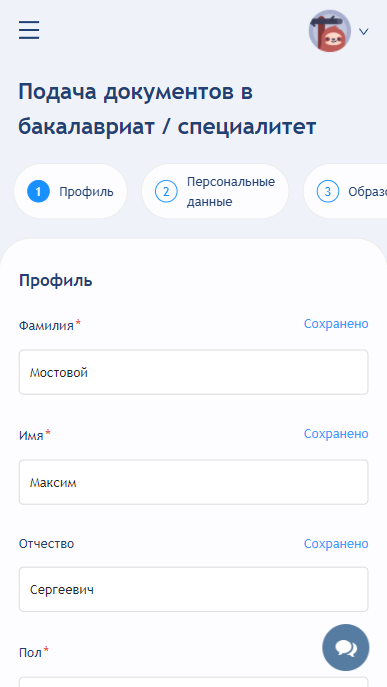
\includegraphics[width=0.5\hsize]{fig/profile-step.png}\\[2mm]
\caption{Форма для заполнения профиля абитуриента}\label{fig:profilestep}
\end{center}
\end{figure}

\subsection{Реализация этапа заполнения персональных данных абитуриента}

На данном этапе, пользователь должен ввести свои паспортные данные, загрузить сканы разворота паспорта с фотографией и разворота паспорта с пропиской, заполнить адрес постоянной регистрации и адрес проживания (рисунок \ref{fig:personaldata}).

\begin{figure}[H]
\begin{center}
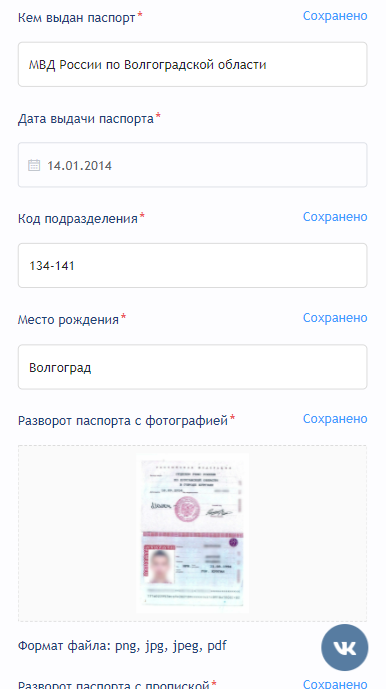
\includegraphics[width=0.5\hsize]{fig/passport.png}\\[2mm]
\caption{Форма для заполнения персональных данных}\label{fig:personaldata}
\end{center}
\end{figure}

Для удобства заполнения адреса постоянной регистрации и адреса проживания, используется сервис содержащий сведения об адресах и о реквизитах документов о присвоении, об изменении, аннулировании адреса (REST-API ФИАС). Первоначально, по запросу к API загружаются все регионы Российской Федерации, далее, запросы строятся на основе данных, которые вводит пользователь (листинг \ref{ls:getadress}).

\begin{lstlisting}[caption={Метод реализующий генерацию запросов в API сервиса ФИАС}, label={ls:getadress}]
getAddress = async (type = 1, regionCode = '', areaCode = '', cityCode = '', villageCode='') => {
  try {
    return await axios.get(`${API_URL}get-objects?
      type=${type}&regionCode=${regionCode}&areaCode=${areaCode}&cityCode=${cityCode}&villageCode=${villageCode}`,
      { headers: authHeader() });
  } catch (error) {
    throw new Error('CLADER API access denied');
  }
}
\end{lstlisting}

Для отображения большого массива данных внутри поля выбора \verb|select|, используется виртуальная прокрутка, элементы содержащие данные переиспользуются, подгружая только новые данные для отображения, таким образом, количество элементов внутри HTML документа остается одинаковым (рисунок \ref{fig:virtualselect}) \cite{algoritm}. Также, внутри поля выбора адреса используется нечеткий поиск, благодаря которому, пользователь может отфильтровать данные в представленном списке. 

По умолчанию, выбрано, что адрес постоянной регистрации совпадает с адресом проживания, в таком случае, введенные данные для адреса регистрации будут использованы и для адреса проживания, иначе, пользователю необходимо отдельно указать данные проживания (рисунок \ref{fig:adressinput}).

\begin{figure}[H]
\begin{center}
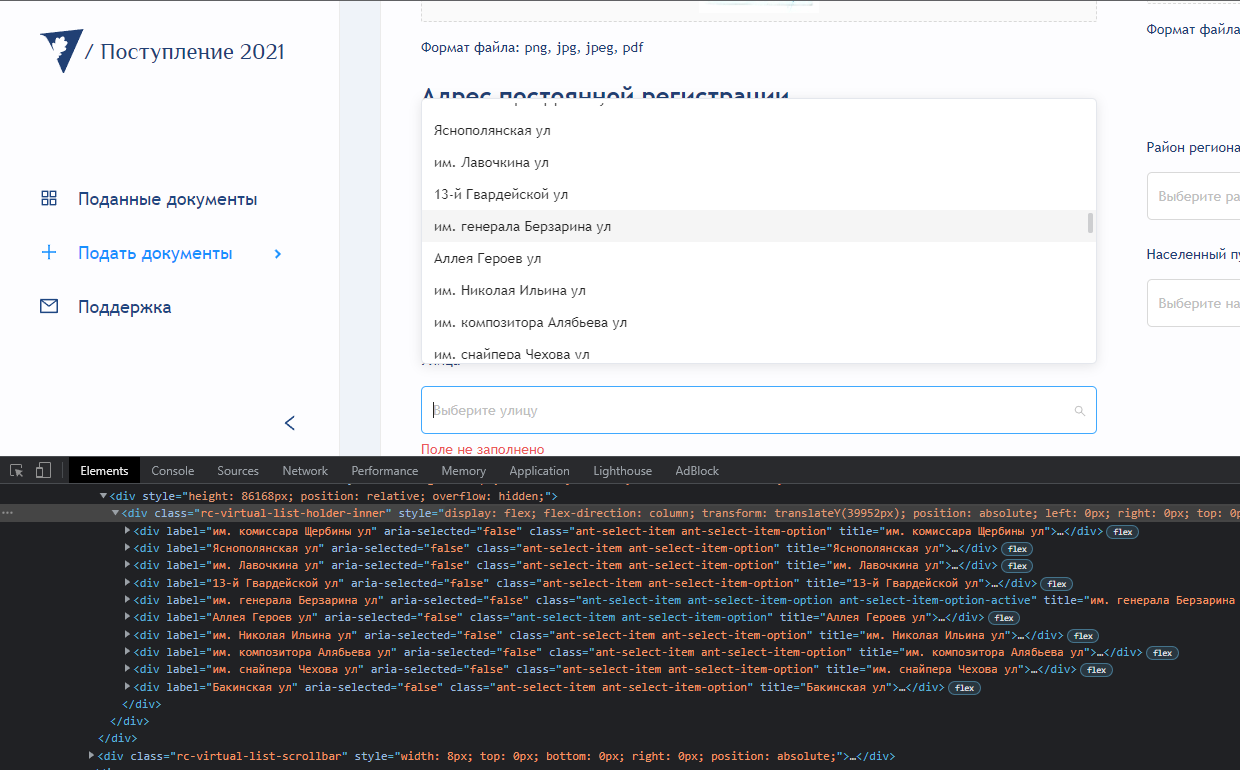
\includegraphics[width=0.9\hsize]{fig/virtual-select.png}\\[2mm]
\caption{Демонстрация работы поля select с виртуальной прокруткой}\label{fig:virtualselect}
\end{center}
\end{figure}

\begin{figure}[H]
\begin{center}
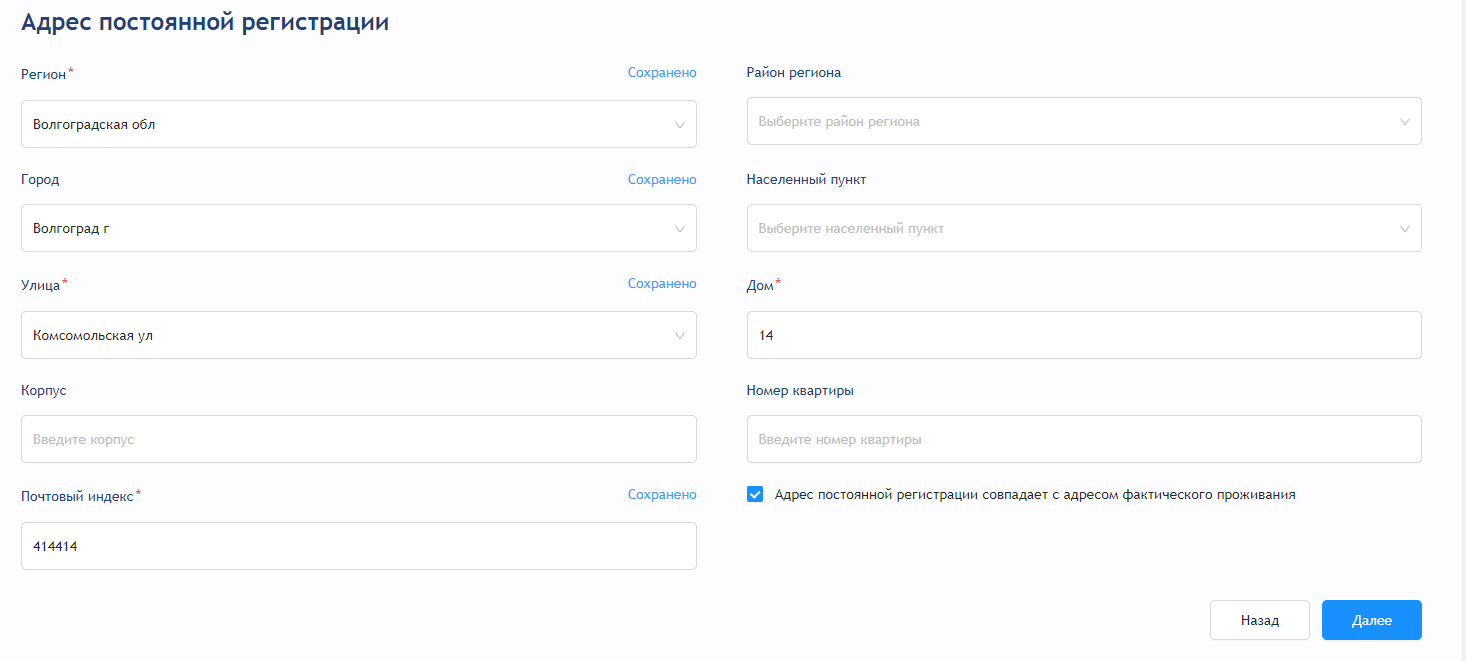
\includegraphics[width=0.9\hsize]{fig/address-input.png}\\[2mm]
\caption{Форма для заполнения адреса постоянной регистрации}\label{fig:adressinput}
\end{center}
\end{figure}

\subsection{Реализация этапа заполнения образования абитуриента}

На данном этапе, пользователь заполняет информацию об образовании, на основании которого он желает подать заявление на поступление. 

С помощью запроса к API, в поле «уровень образования» загружаются списки уровней образования, полученные из справочника, после выбора уровня образования, с помощью запроса к API, в поле «тип документа» загрузятся списки документов, соответствующие выбранному уровню образования. После чего, абитуриент должен заполнить оставшиеся поля, загрузить скан документа об образовании и скан приложения с оценками (рисунок \ref{fig:educationform}).

\begin{figure}[H]
\begin{center}
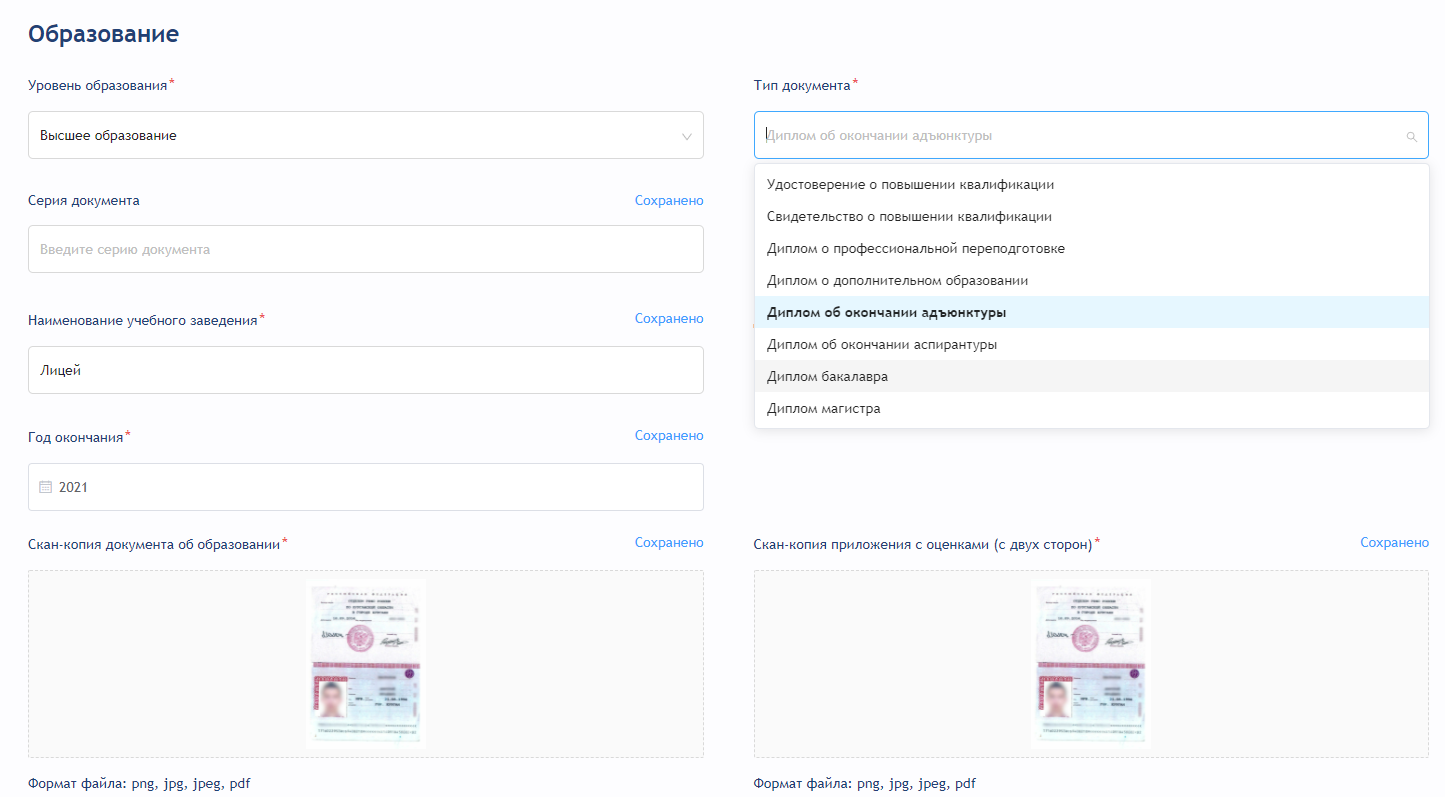
\includegraphics[width=0.9\hsize]{fig/edu.png}\\[2mm]
\caption{Форма для заполнения образования}\label{fig:educationform}
\end{center}
\end{figure}

\subsection{Реализация этапа заполнения достижений и льгот абитуриента}

На данном этапе, абитуриент может загрузить свои индивидуальные достижения, целевые договоры, олимпиады, льготы, данный этап является необязательным к заполнению и заполняется по желанию абитуриента.

Для добавления индивидуального достижения, абитуриенту необходимо загрузить скан подтверждающего документа, после отправки заявления, оно будет проверено приемной комиссией и соответствующие баллы за индивидуальное достижение будут добавлены.

Для добавления целевого договора, абитуриенту необходимо заполнить номер договора, наименование организации, кем выдан договор, дату выдачи, и загрузить скан подтверждающего документа (рисунок \ref{fig:dogovor}). Добавленные целевые договоры будут загружены, при поступлении на направление с целевым приемом.

\begin{figure}[H]
\begin{center}
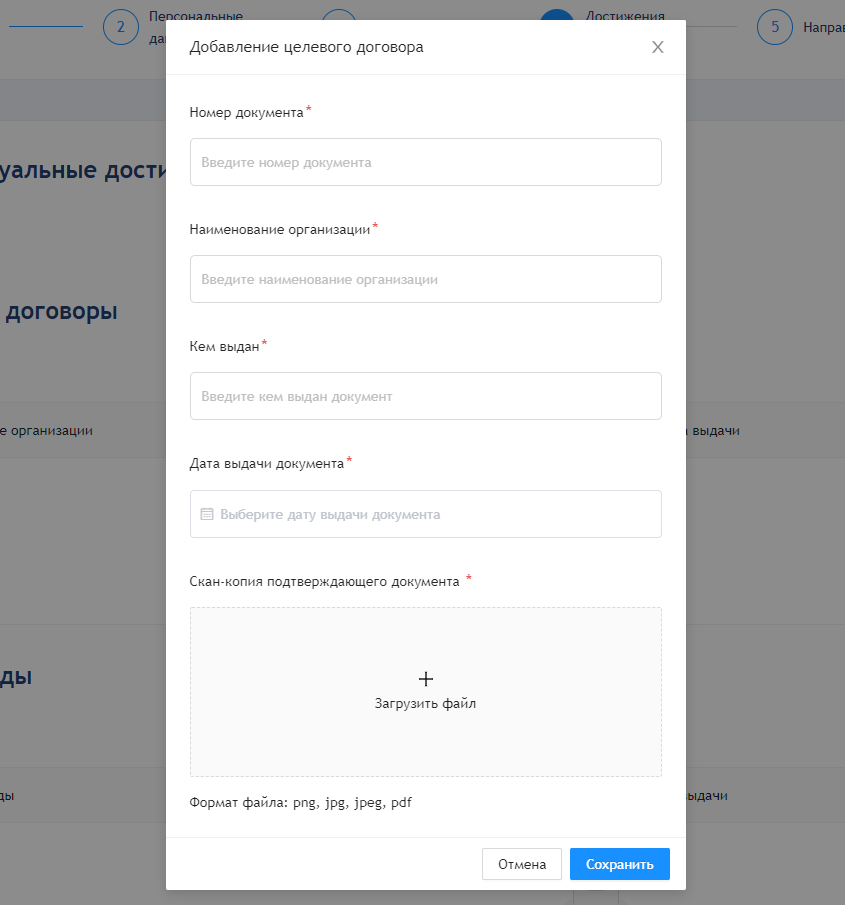
\includegraphics[width=0.9\hsize]{fig/dogovor.png}\\[2mm]
\caption{Добавление целевого договора}\label{fig:dogovor}
\end{center}
\end{figure}

Для добавления олимпиады, абитуриент должен выбрать тип олимпиады и класс, предоставляемые списки загружаются по запросу к API. Далее, необходимо заполнить номер документа, серию документа, кем выдан документ, дату выдачи, и загрузить скан подтверждающего документа. Добавленные олимпиады будут загружены, при выборе поступления без вступительных испытаний.

Для добавления льготы, абитуриент должен выбрать тип льготы из предоставленного списка, который загружается по запросу к API (листинг \ref{ls:getprivilegy}). Далее, необходимо заполнить номер документа, серию документа, кем выдан документ, дату выдачи, и загрузить скан подтверждающего документа.

\begin{lstlisting}[caption={Метод загружающий список список типов льгот}, label={ls:getprivilegy}]
UserService.getPrivilegeTypes().then(
  response => {
    if (response.data.result.status) {
      // eslint-disable-next-line no-unused-vars
      this.dict_privilege_code = response.data.result.model

      Object.entries(response.data.result.model).forEach(([key, value]) => {
        this.form.privilege_code.options.push({
          value: key,
          label: value,
        });
      });
      this.form.privilege_code.isLoading = false;
    } else {
      this.$store.dispatch('auth/logout');
      this.$router.push('/login');
    }
  },
  error => {
    this.content = (error.response && error.response.data && error.response.data.message) || error.message || error.toString();
  }
);
\end{lstlisting}

\subsection{Реализация этапа выбора направлений для поступления}

На данном этапе, абитуриент должен выбрать направления для поступления. Ограничение на количество выбранных направлений отличается в зависимости от уровня образования. С точки зрения пользователя, компонент \verb|LkPrograms.vue| имеет две вкладки, вкладку с выбранными направлениями и вкладку с выбором направлений.

Доступные направления загружаются по запросу к API, в зависимости от уровня образования, который определяется по номеру заявления. Все направления и укрупненные группы представлены в виде карточек, содержащих в себе название конкурсной группы, профиль, институт к которому принадлежит конкурсная группа, форма обучение, и форму оплаты, так же, укрупненные конкурсные группы содержат список направлений, которые входят в укрупненную конкурсную группу (рисунок \ref{fig:choiceprogram}).

Для выбора направления для поступления, необходимо нажать на карточку с направлением, после чего, по нажатию кнопки «добавить», все отмеченные направления будут перемещены в выбранные, а пользователь будет автоматически перенаправлен на вкладку с выбранными направлениями.

\begin{figure}[H]
\begin{center}
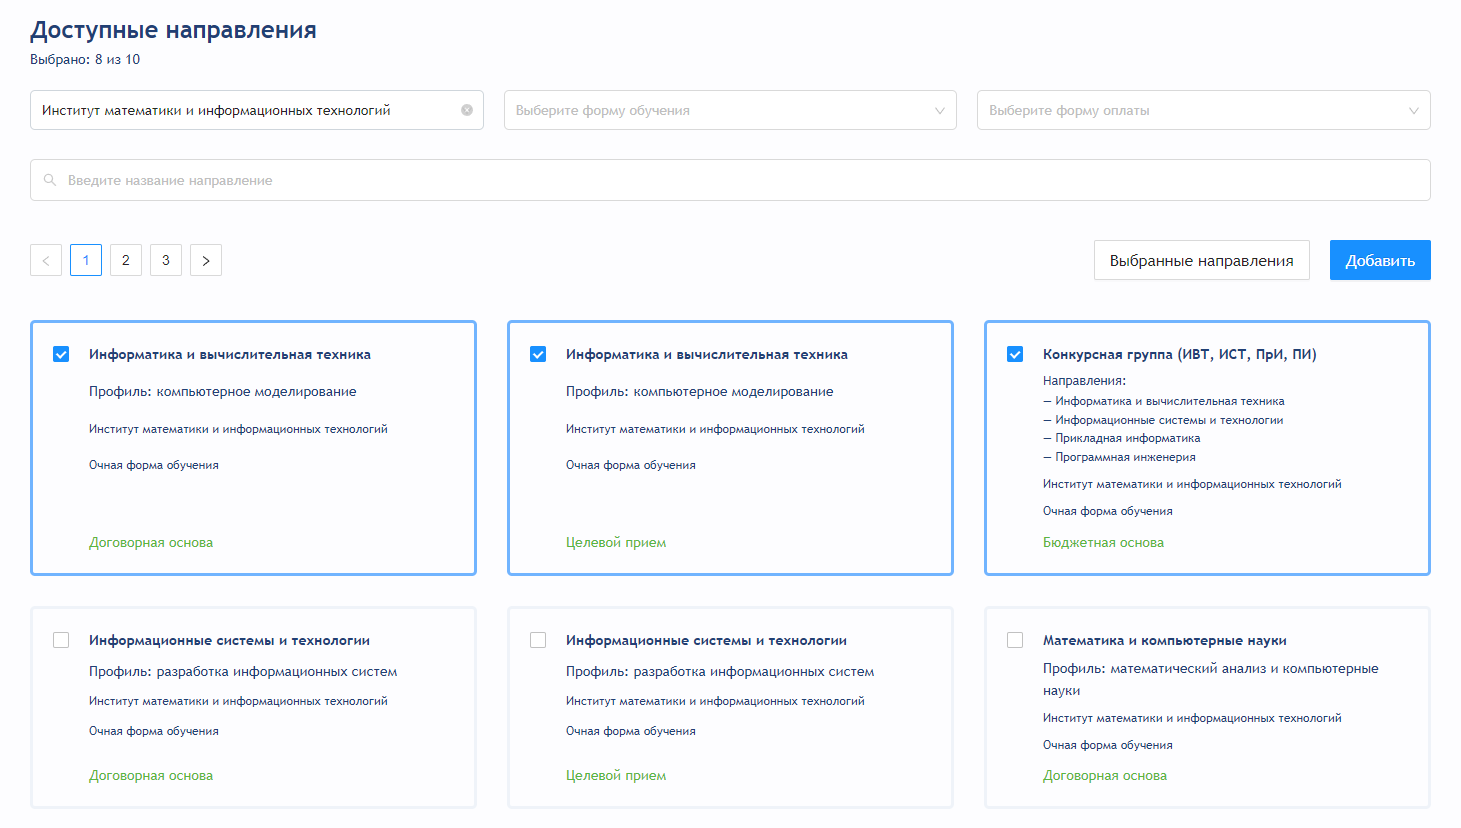
\includegraphics[width=0.9\hsize]{fig/choice-program.png}\\[2mm]
\caption{Форма выбора направлений для поступления}\label{fig:choiceprogram}
\end{center}
\end{figure}

Поскольку, количество доступных направлений может быть очень велико, была реализована фильтрация и нечеткий поиск по конкурсным группам. Реализованы фильтры по институтам, форме обучения, форме оплаты, нечеткий поиск с подсказками ищет совпадения по названию конкурсных группы, а также по направлениям входящих в укрупненную конкурсную группу (рисунок \ref{fig:choiceprogramfilter}).

\begin{figure}[H]
\begin{center}
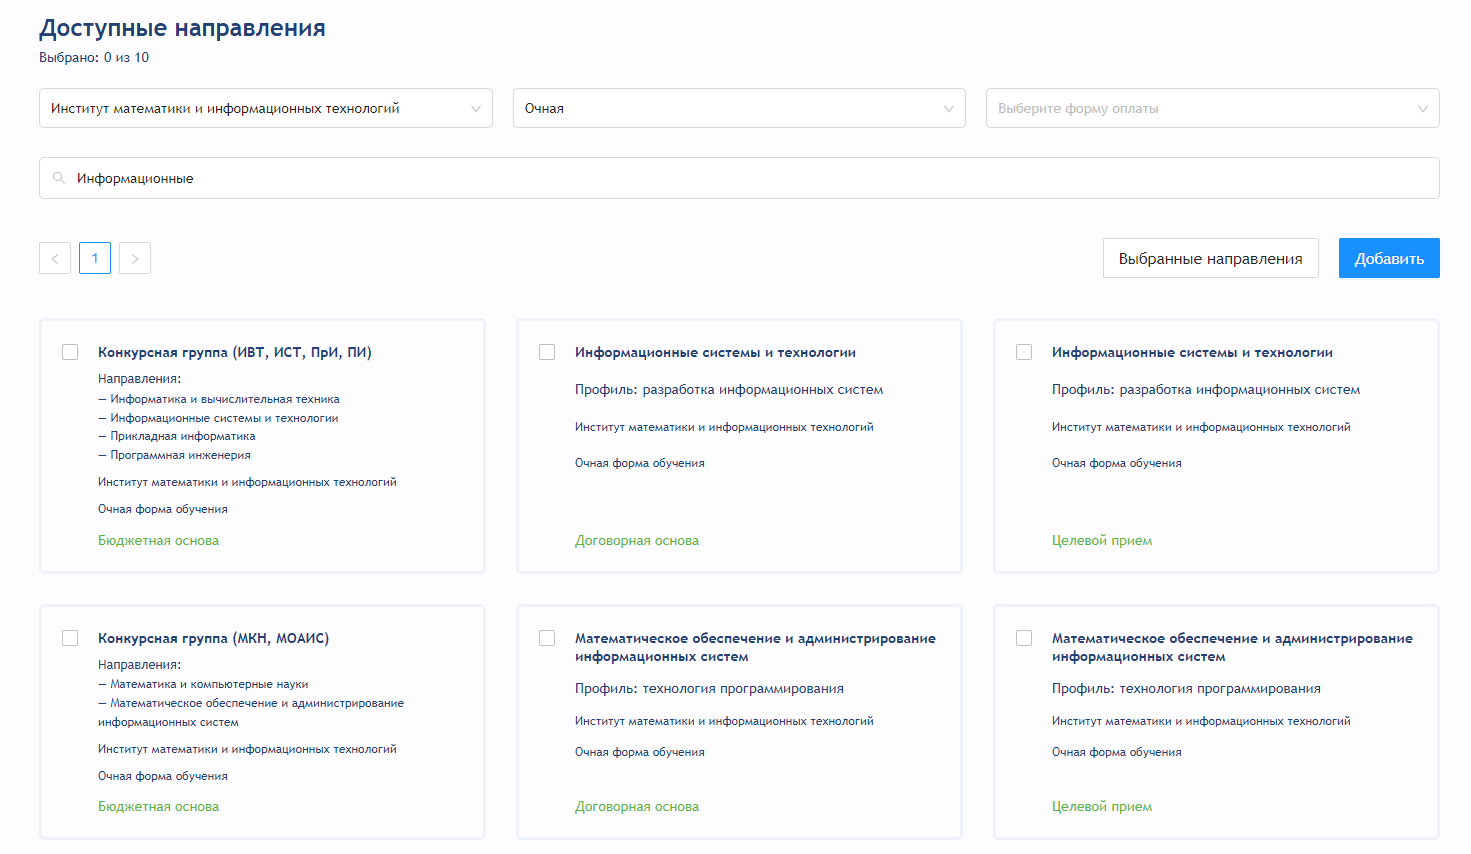
\includegraphics[width=0.9\hsize]{fig/programms.png}\\[2mm]
\caption{Пример работы фильтрации и нечеткого поиска по конкурсным группам}\label{fig:choiceprogramfilter}
\end{center}
\end{figure}

После того, как абитуриент выбрал направления для поступления, он может расставить приоритеты выбранных направлений, для этого необходимо перетащить нужное направление по вертикальной оси, приоритет направлений расставляется снизу-вверх (рисунок \ref{fig:changepriority}) (листинг \ref{ls:prioritychange}).

\begin{figure}[H]
\begin{center}
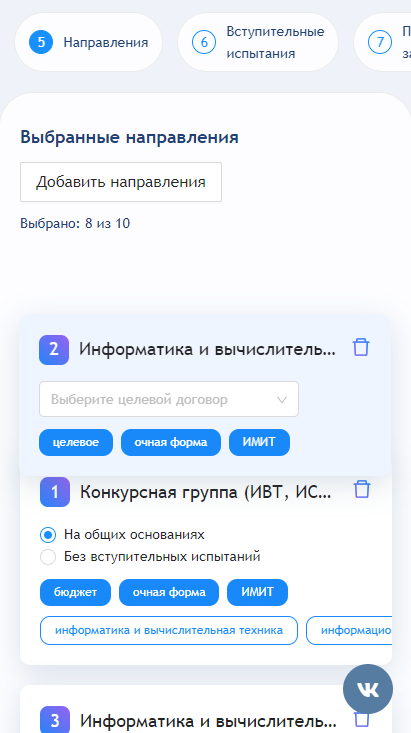
\includegraphics[width=0.5\hsize]{fig/change-priority-programs.png}\\[2mm]
\caption{Пример изменения приоритета направления}\label{fig:changepriority}
\end{center}
\end{figure}

\begin{lstlisting}[caption={Вычисляемое свойство реализующие изменение приоритета направлений}, label={ls:prioritychange}]
const dragOptions = computed(() => ({
  sort: true,
  animation: 200,
  group: 'description',
  disabled: false,
  ghostClass: 'direction-selected-ghost',
  chosenClass: 'direction-selected-chosen',
  dragClass: 'direction-selected-drag',
  forceFallback: true,
  fallbackClass: 'direction-selected-fallback',
  fallbackOnBody: false,
  fallbackTolerance: 7,
  delay: 200, // time in milliseconds to define when the sorting should start
  delayOnTouchOnly: true, // only delay if user is using touch
  onChange(evt) {
    directionsSelectedList.value[evt.moved.newIndex].place = evt.moved.newIndex + 1;
    placeSave(evt.moved.element.directionInfo.code, evt.moved.newIndex + 1);
    console.log(evt);

    directionsSelectedList.value.slice(evt.moved.oldIndex < evt.moved.newIndex ? evt.moved.oldIndex : evt.moved.newIndex + 1,
      evt.moved.oldIndex < evt.moved.newIndex ? evt.moved.newIndex : evt.moved.oldIndex + 1)
      .forEach(value => {
        if (evt.moved.oldIndex < evt.moved.newIndex) {
          value.place -= 1;
          placeSave(value.directionInfo.code, value.place - 1);
        } else {
          value.place += 1;
          placeSave(value.directionInfo.code, value.place + 1);
        }
      });
  },
}));
\end{lstlisting}

Так же, на странице выбранных направлений, абитуриент может выбрать форму поступления по каждому направлению, в случае выбора поступления без вступительных испытаний, абитуриент должен выбрать добавленную на прошлом этапе льготу (рисунок \ref{fig:choiceprivilegy}). В случае выбора конкурсной группы с формой оплаты по целевому договору, абитуриент должен выбрать добавленный на прошлом этапе целевой договор.

\begin{figure}[H]
\begin{center}
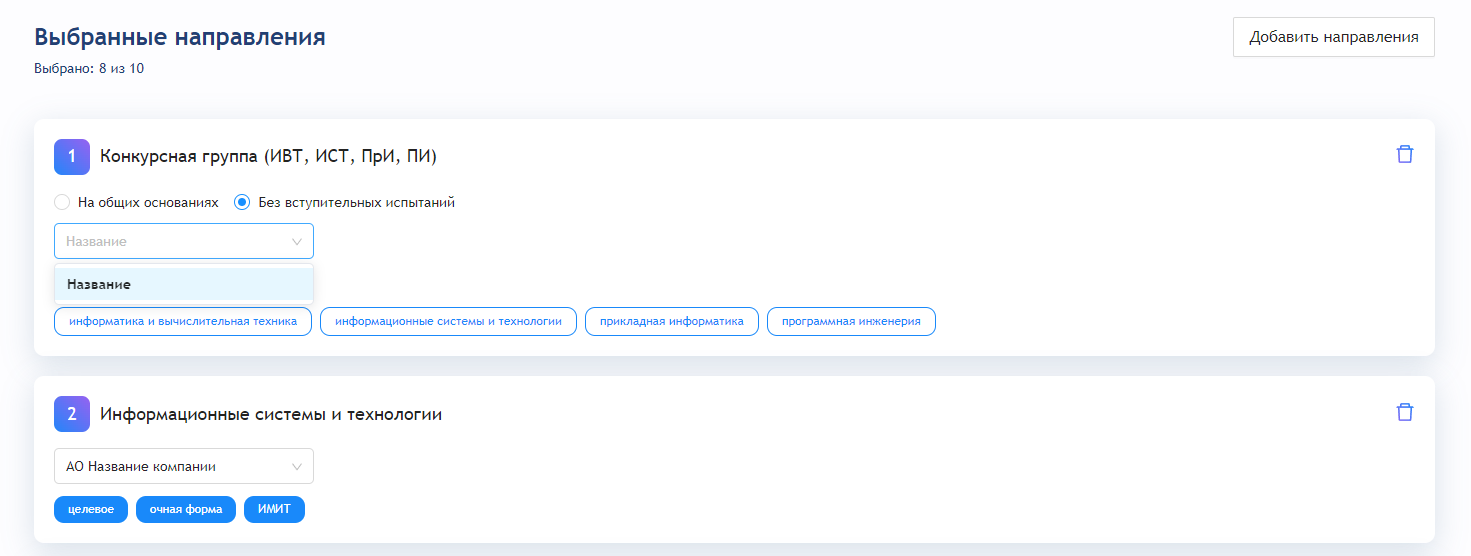
\includegraphics[width=0.9\hsize]{fig/choice-privilegy.png}\\[2mm]
\caption{Пример применения льгот и целевых договоров к направлению}\label{fig:choiceprivilegy}
\end{center}
\end{figure}

\subsection{Реализация этапа заполнения вступительных испытаний}

На данном этапе, абитуриент должен выбрать и ввести вступительные испытания для всех выбранных направлений. Для каждого направления, с помощью запроса к API, загружаются обязательные дисциплины, а также список дисциплин по выбору (листинг \ref{ls:egelist}), так же рядом с каждой дисциплиной указывается минимальный балл, необходимый для поступления (рисунок \ref{fig:egescore}).

\begin{figure}[H]
\begin{center}
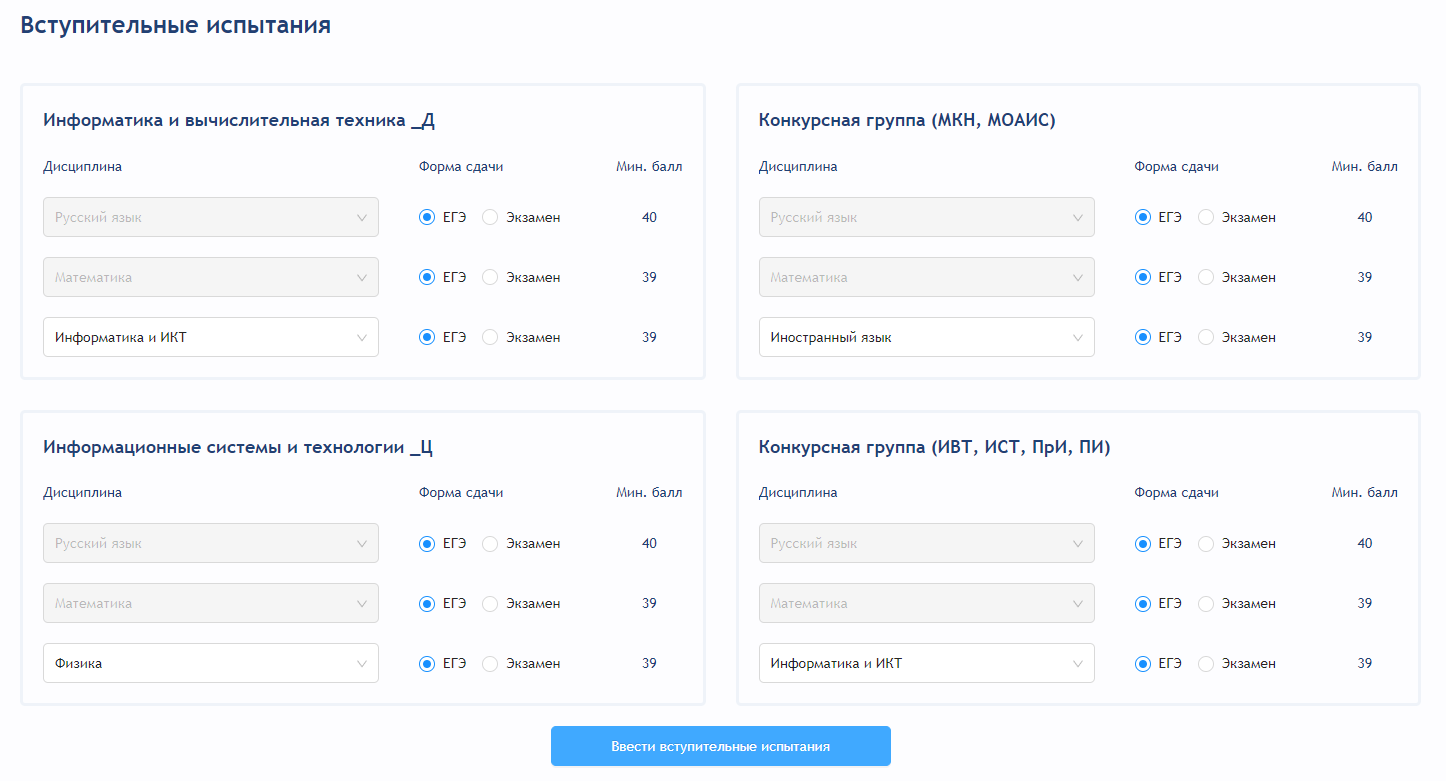
\includegraphics[width=0.9\hsize]{fig/input-ege-score.png}\\[2mm]
\caption{Форма выбора вступительных испытаний}\label{fig:egescore}
\end{center}
\end{figure}

\begin{lstlisting}[caption={Метод загружающий список вступительных испытаний}, label={ls:egelist}]
const getEntrances = async () => {
  const response = await StatementService.getExams(await getStatementId());
  console.log(response.data.result);
  if (response.data.result.model) {
    response.data.result.model.forEach(item => {

      const entranceTmp = {
        statementName: item.name,
        id: item.id,
        entrances: [],
      };

      item.set.forEach(value => {
        const entranceOptions = [];
        value.forEach(entrance => {
          entranceOptions.push({
            value: entrance.discipline_id,
            label: entrance.discipline_name,
            minScore: entrance.minimal_balls,
          });
        });

        entranceTmp.entrances.push({
          disciplinesOptions: entranceOptions,
          disciplinesSelected: entranceOptions[0].value,
          disciplinesSelectedLabel: entranceOptions[0].label,
          disciplinesSaved: false,
          disciplinesErrors: [],
          deliveryOptions: value[0].forms,
          deliverySelected: value[0].forms[0].value,
          deliverySelectedLabel: value[0].forms[0].label,
          deliverySaved: false,
          deliveryErrors: [],
          minScore: entranceOptions[0].minScore,
        });
      });

      entranceList.value.push(entranceTmp);
    });
  } else {
    programsNotSelected.value = true;
  }
};
\end{lstlisting}

После того, как пользователь указал нужные дисциплины, он должен ввести результаты вступительных испытаний вы выбранным дисциплинам (рисунок \ref{fig:egescoreinput}).

\begin{figure}[H]
\begin{center}
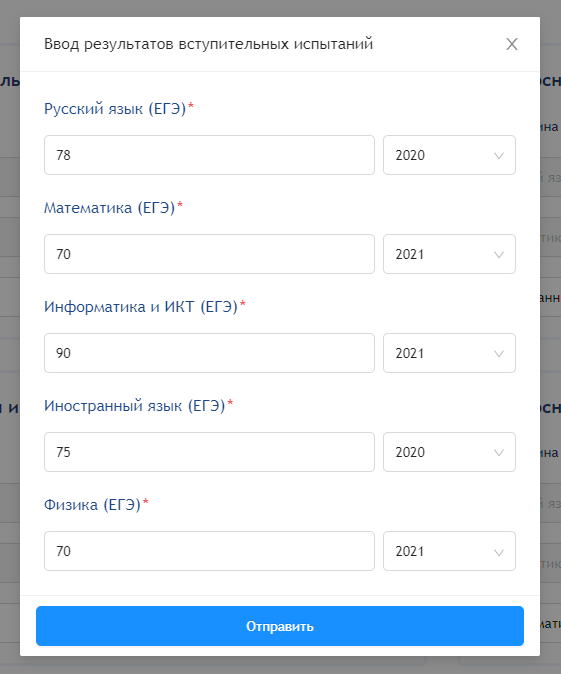
\includegraphics[width=0.6\hsize]{fig/ege-input-result.png}\\[2mm]
\caption{Форма ввода результатов вступительных испытаний}\label{fig:egescoreinput}
\end{center}
\end{figure}

\subsection{Реализация этапа подачи заявления на поступление}

На последнем этапе, абитуриент должен скачать автоматических сформированные бланки всех документов (рисунок \ref{fig:statement}), подписать их, и загрузить их сканы в соответствующие поля. По указанной дате рождения, определяется возраст поступающего в случае, если указанный возраст меньше восемнадцати лет, будут сформированы бланки для несовершеннолетнего абитуриента.

\begin{figure}[H]
\begin{center}
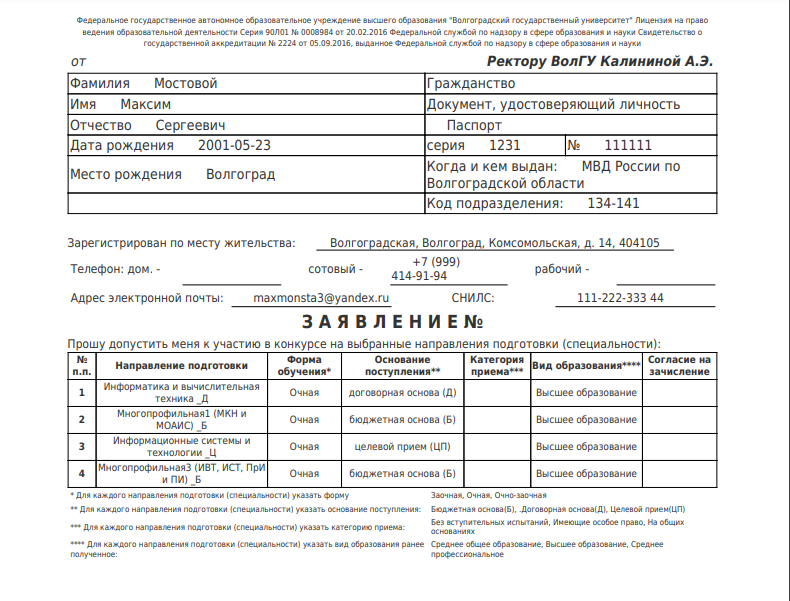
\includegraphics[width=0.9\hsize]{fig/statement.png}\\[2mm]
\caption{Сформированное заявление на поступление}\label{fig:statement}
\end{center}
\end{figure}

Так же, перед отправкой заявления, все заполненные данные проходят дополнительную валидацию на стороне сервера в случае, если какие-то поля были пропущены, пользователь получит соответствующие сообщение об ошибке (листинг \ref{ls:sendstatement}).

\begin{lstlisting}[caption={Валидация всех полей и отправка заявления}, label={ls:sendstatement}]
handleClick() {
  BachelorService.checkSendStatementStatus()
    .then(response => {
      if (response.data.result.status) {
        this.$router.replace({name: 'SubDocSuccessView'});
      } else {
        this.errors = response.data.result.error;
      }
    })
    .catch(error => {
      alert('Input all fields!')
      console.log(error)
    });
},
\end{lstlisting}

В случае успешного прохождения валидации, пользователь будет перенаправлен на специальную страницу, с сообщением о том, что его заявление успешно отправлено на проверку приемной комиссии (рисунок \ref{fig:statementsuccsess}). Статус заявления измениться на «отправлено».  В случае, если абитуриент захочет отредактировать отправленное заявление, его статус будет автоматических сброшен на статус «формируется».

\begin{figure}[H]
\begin{center}
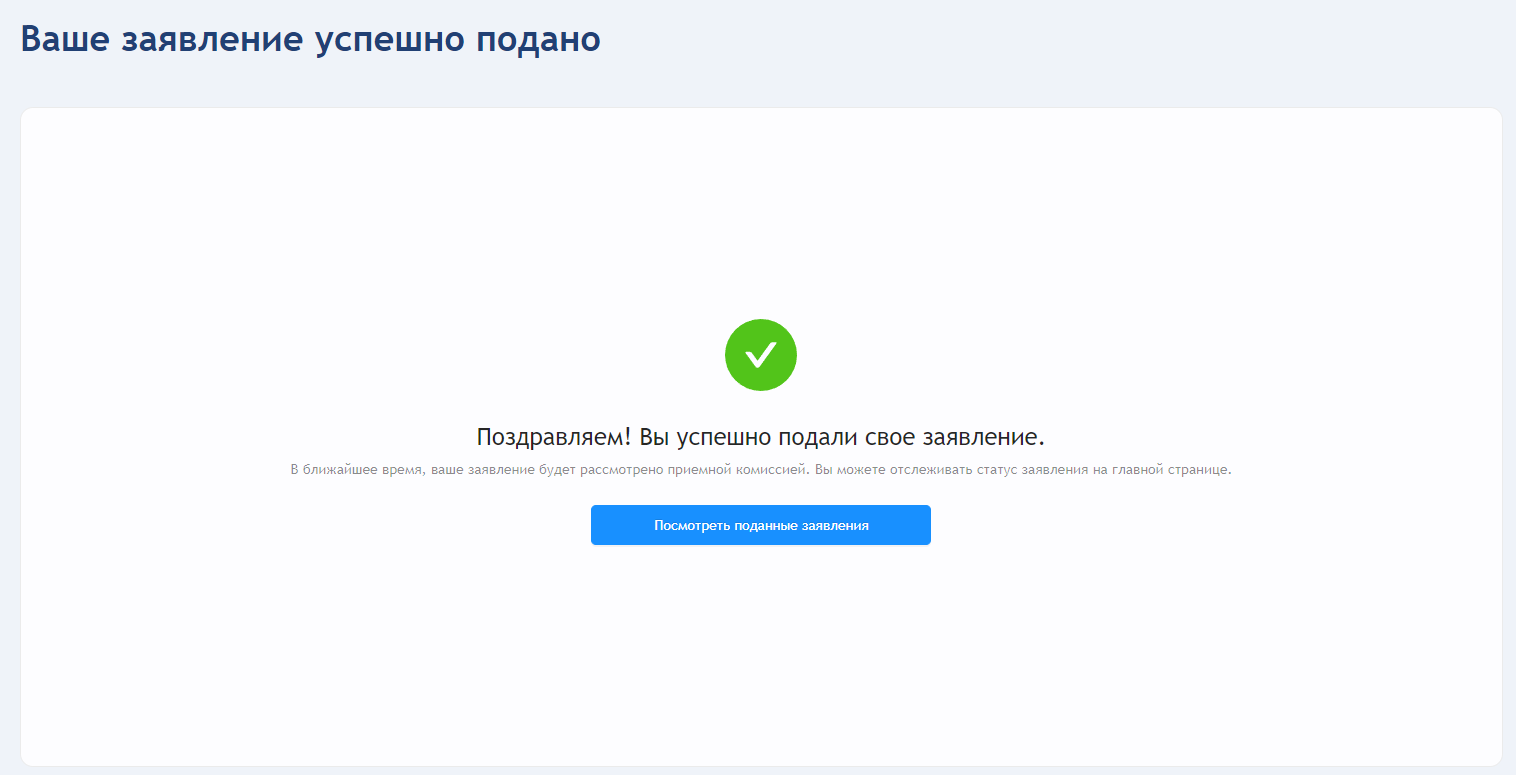
\includegraphics[width=0.9\hsize]{fig/statement-succsess.png}\\[2mm]
\caption{Страница с информацией о том, что заявление успешно подано}\label{fig:statementsuccsess}
\end{center}
\end{figure}

\section{Реализация процесса подачи согласия на зачисление}

\subsection{Подача согласия на зачисление}

После того, как сотрудник приемной комиссии одобрит отправленное заявление, абитуриент может подать согласие на зачисление. Согласие на зачисление подается на одно из выбранных направлений, указанных в заявлении. Подать согласие на зачисление можно ограниченное количество раз, перед подачей согласия, абитуриенту отображается количество оставшихся попыток (рисунок \ref{fig:agreestart}).

\begin{figure}[H]
\begin{center}
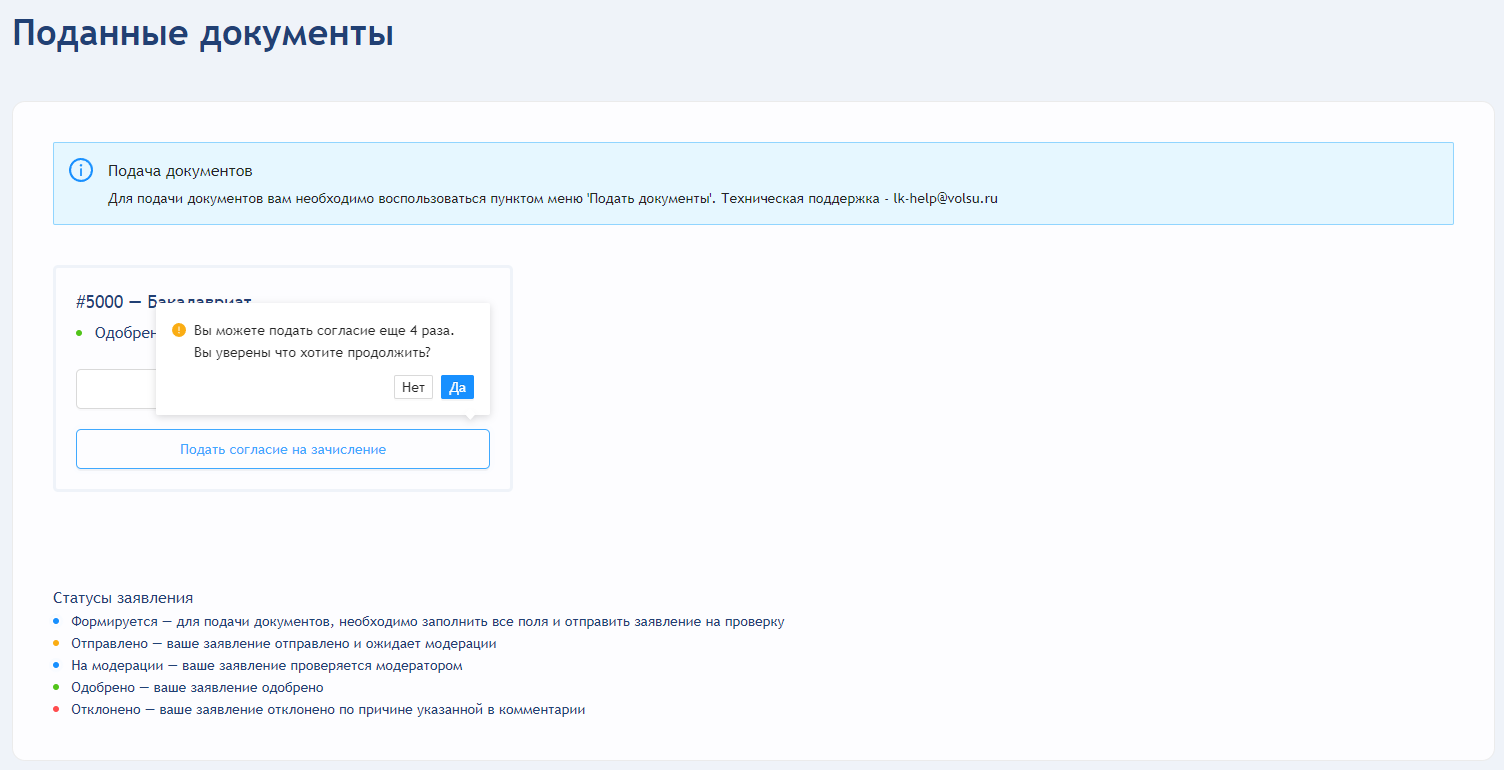
\includegraphics[width=0.9\hsize]{fig/agree-start.png}\\[2mm]
\caption{Подача согласия на зачисление}\label{fig:agreestart}
\end{center}
\end{figure}

После выбора направления, для подачи согласия, для абитуриента автоматических формируется перезаполненный бланк (рисунок \ref{fig:agreedoc}), который он должен подписать, и загрузить скан бланка в соответствующие поле (рисунок \ref{fig:agresend}).

\begin{figure}[H]
\begin{center}
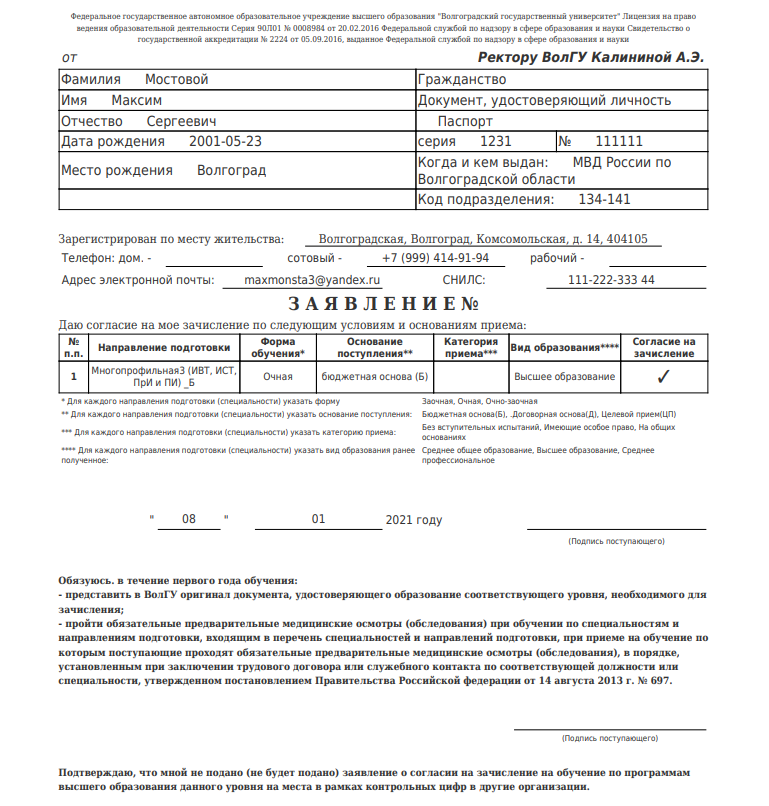
\includegraphics[width=0.9\hsize]{fig/agree-doc.png}\\[2mm]
\caption{Сформированный бланк согласия на зачисление}\label{fig:agreedoc}
\end{center}
\end{figure}

\begin{figure}[H]
\begin{center}
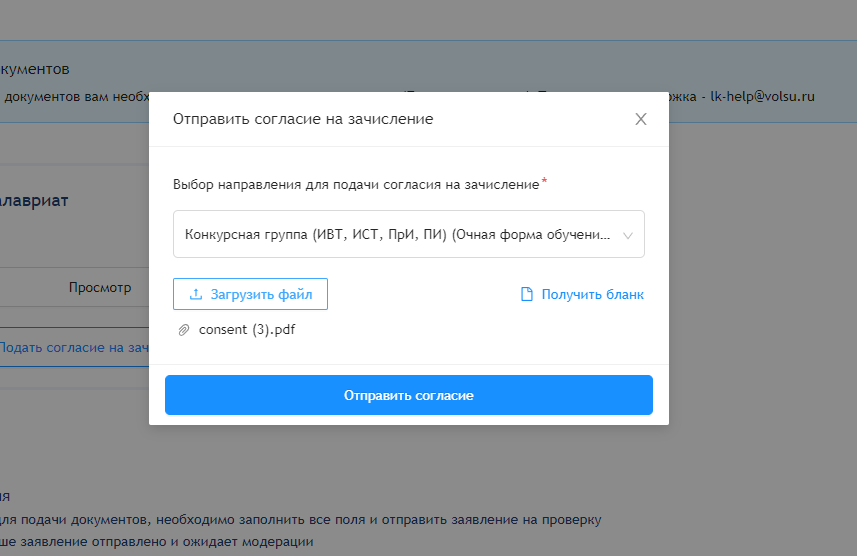
\includegraphics[width=0.9\hsize]{fig/agree-send.png}\\[2mm]
\caption{Отправка согласия на выборное направление}\label{fig:agresend}
\end{center}
\end{figure}

После того, как согласие будет одобрено сотрудником приемной комиссии и занесено в систему учета, абитуриент найти себя в рейтинге абитуриента (рисунок \ref{fig:agreerating}).

\begin{figure}[H]
\begin{center}
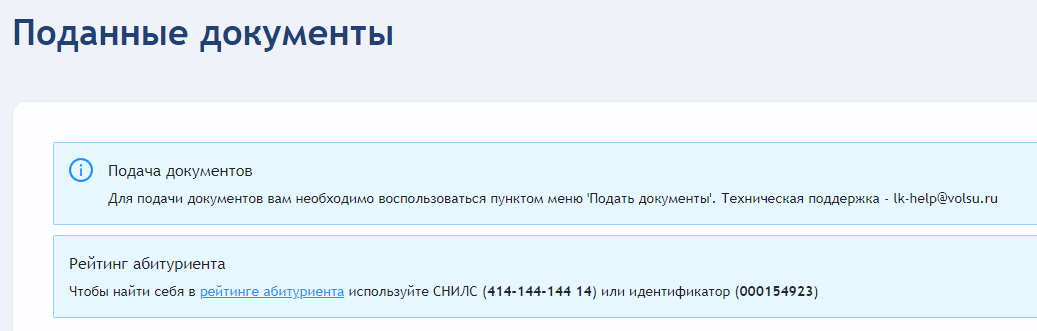
\includegraphics[width=0.9\hsize]{fig/agree-rating.png}\\[2mm]
\caption{Сообщение о том, как абитуриенту найти себя в рейтинге абитуриентов}\label{fig:agreerating}
\end{center}
\end{figure}

До момента одобрения согласия на зачисление сотрудником приемной комиссии, абитуриент может удалить согласие на зачисление, в таком случае, он сможет подать новое согласие на зачисление, без утраты попытки (рисунок \ref{fig:agreedelete}).

\begin{figure}[H]
\begin{center}
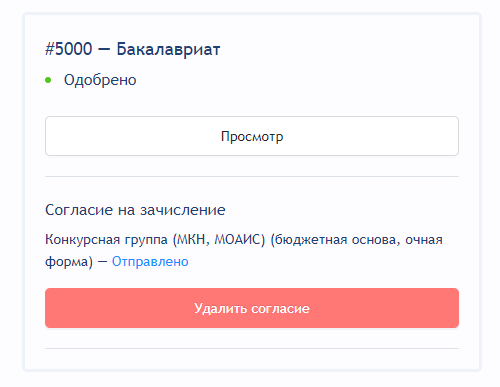
\includegraphics[width=0.7\hsize]{fig/agree-delete.png}\\[2mm]
\caption{Удаление согласия на зачисление}\label{fig:agreedelete}
\end{center}
\end{figure}

\subsection{Отзыв согласия на зачисление}

В случае, если абитуриент хочет по какой-либо причине отозвать уже одобренное согласие, он должен подписать автоматически сформированный бланк отзыва (рисунок \ref{fig:agreecanceldoc}) согласия и загрузить его в соответствующие поле. Отзыв согласия должен быть одобрен сотрудником приемной комиссии. После одобрения отзыва согласия, абитуриент может снова подать согласие на зачисление, в рамках оставшихся попыток.

\begin{figure}[H]
\begin{center}
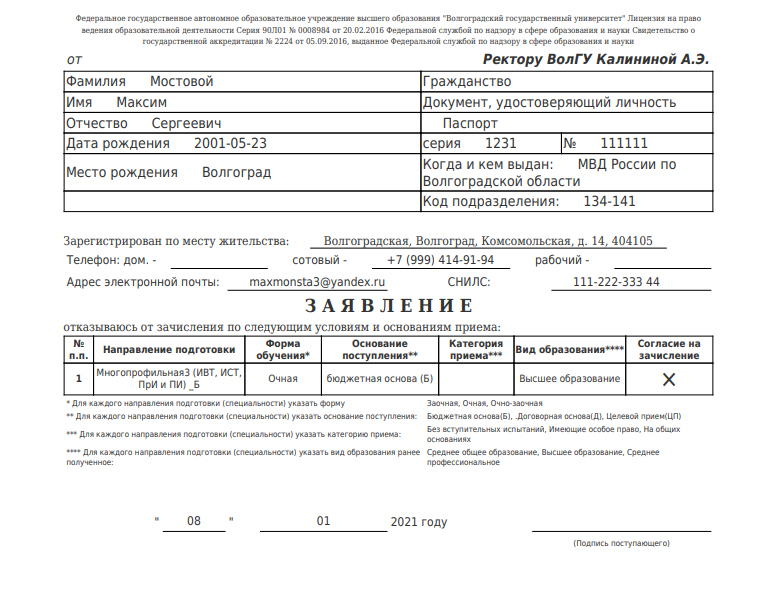
\includegraphics[width=0.9\hsize]{fig/agree-cancel.png}\\[2mm]
\caption{Сформированный бланк отзыва согласия на зачисление}\label{fig:agreecanceldoc}
\end{center}
\end{figure}

До момента одобрения отзыва согласия сотрудником приемной комиссии, абитуриент может удалить отзыв согласия, в таком случае, его согласие на зачисление останется в силе (рисунок \ref{fig:agrecanseledelete}).

\begin{figure}[H]
\begin{center}
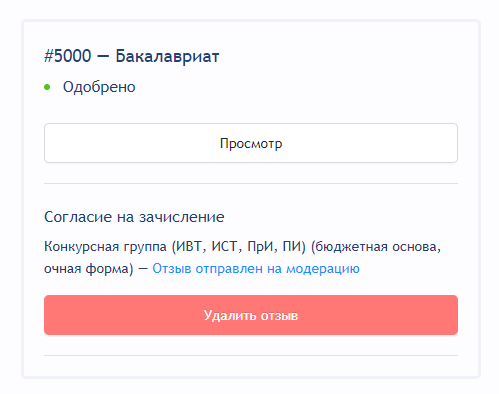
\includegraphics[width=0.7\hsize]{fig/agree-cansel-delete.png}\\[2mm]
\caption{Удаление отзыва согласия на зачисление}\label{fig:agrecanseledelete}
\end{center}
\end{figure}

\section{Реализация функционала обработки заявлений на поступление и согласий на зачисление}

Для сотрудников приемной комиссии создана специальная панель для обработки заявлений на поступление и согласий на зачисление. На сервере хранится информация о сотрудниках приемной комиссии и их правах доступа. Каждый сотрудник может обрабатывать данные согласно своим правам доступа, так, сотрудники обрабатывающие заявления и согласия института математики и информационных технологий, имеют доступ к данным только по своему институту.

Все согласия и заявления представлены в виде таблицы с пагинацией, данные в таблицу динамически загружаются по запросу к API (листинг \ref{ls:moderatorfeath}). В таблице представлена необходимая информация для идентификации заявления или заявления, ответственный, который занимается обработкой отправленного заявления или согласия, и кнопка просмотра полной информации о согласии или заявлении (рисунок \ref{fig:moderatorview}).

\begin{figure}[H]
\begin{center}
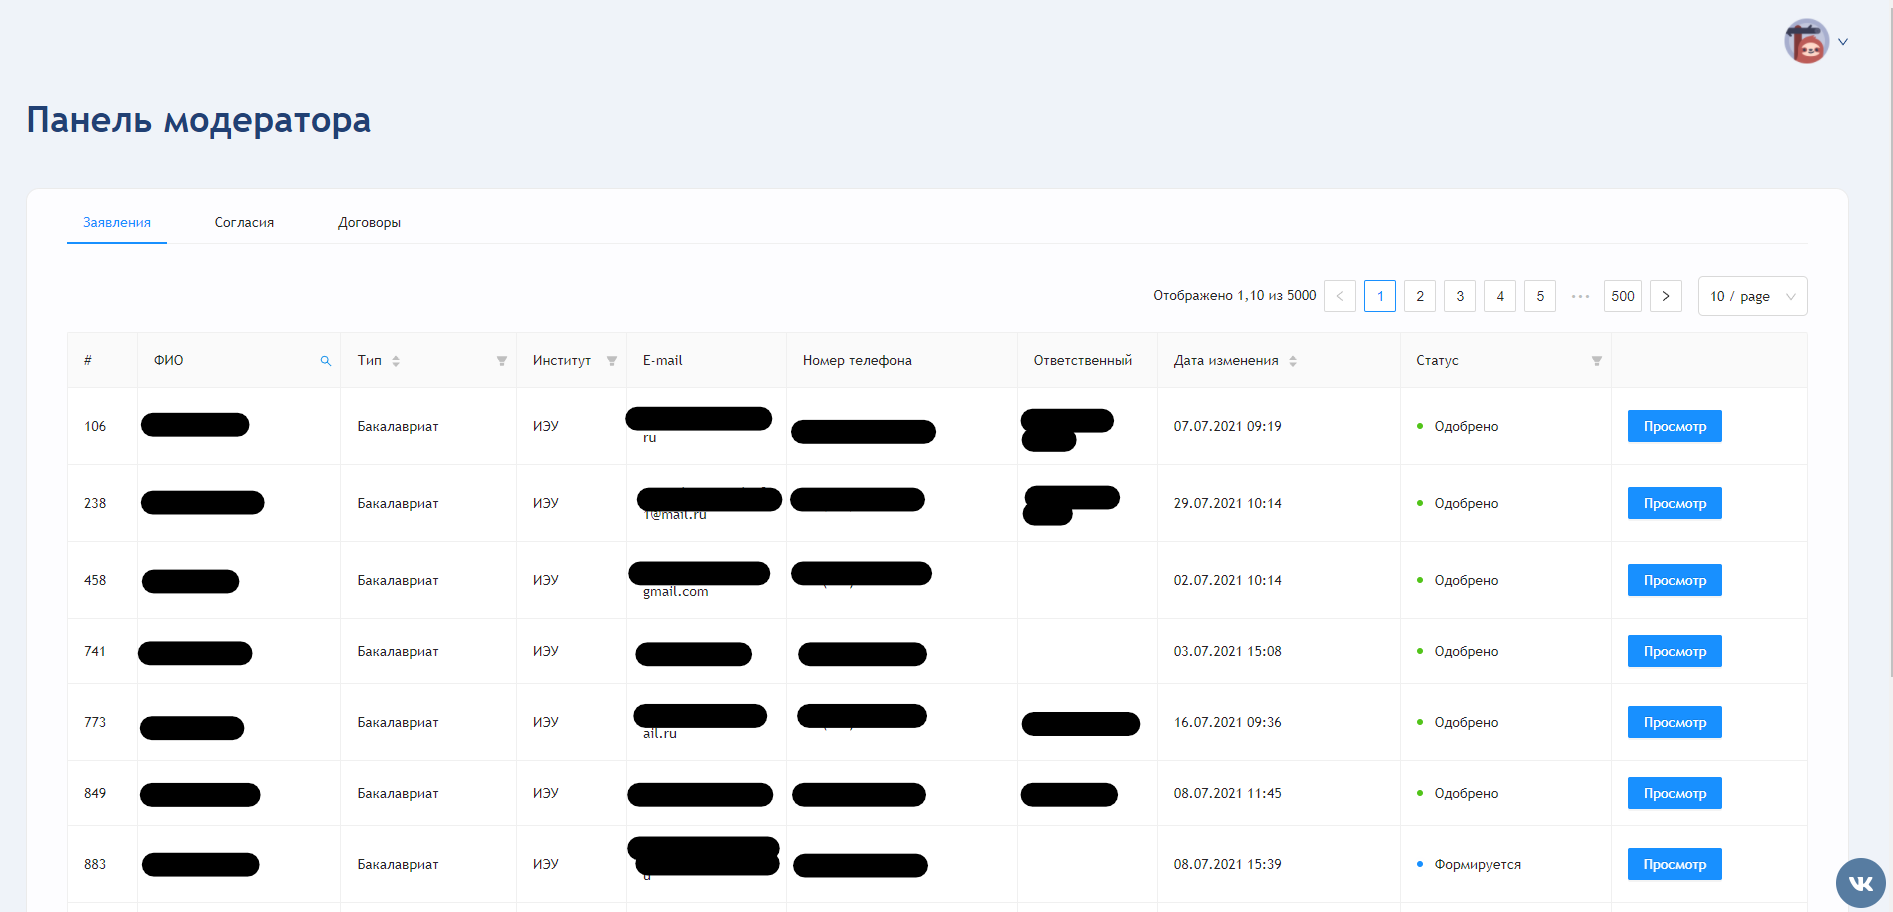
\includegraphics[width=1\hsize]{fig/moderator.png}\\[2mm]
\caption{Панель сотрудника приемной комиссии}\label{fig:moderatorview}
\end{center}
\end{figure}

\begin{lstlisting}[caption={Метод загружающий список заявлений}, label={ls:moderatorfeath}]
fetch(params = {}) {
  this.loading = true;

  ModerationService.getStatements(params).then(
    response => {
      const pagination = {...this.pagination}

      this.data = response.data.results

      pagination.total = response.data.total;

      this.loading = false;
      this.pagination = pagination;
    },
    error => {
      this.content = (error.response && error.response.data && error.response.data.message) || error.message || error.toString();
    }
  );
}
\end{lstlisting}

Каждое согласие или заявление может обрабатывать только один сотрудник приемной комиссии. Сотрудник назначается ответственным на отправленное согласие или заявление при его просмотре в случае, если оно имеет статус «отправлено».

Реализована возможность фильтрации согласий и заявлений по институтам, уровню образования и статусу заявления (рисунок \ref{fig:moderatorfilter}). Конкретное заявление можно найти при помощи нечеткого поиска по ФИО абитуриента. Так же имеется возможность отсортировать данные по уровню образования и дате изменения заявления или согласия.

\begin{figure}[H]
\begin{center}
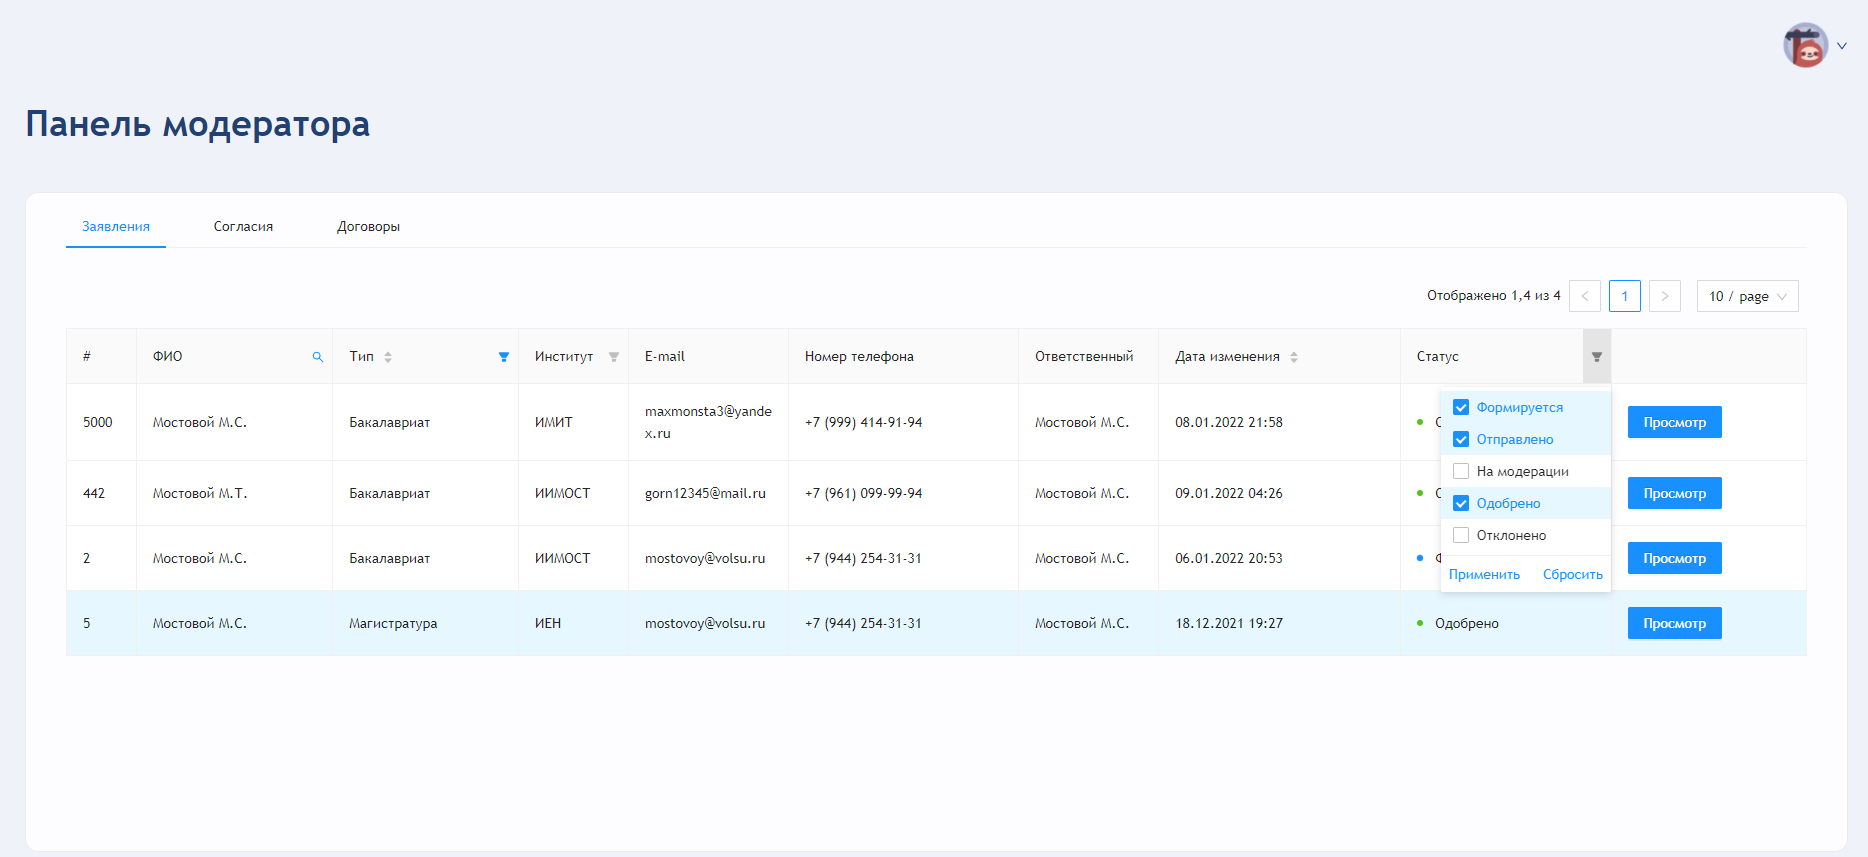
\includegraphics[width=1\hsize]{fig/moderator-filter.png}\\[2mm]
\caption{Пример фильтрации заявлений}\label{fig:moderatorfilter}
\end{center}
\end{figure}

При просмотре полной информации о заявлении, сотрудник приемной комиссии может просмотреть все данные, заполненные абитуриентом, а также загрузить все прикрепленные файлы (рисунок \ref{fig:moderatorstatementview}). Первоначально, сотрудник приемной комиссии должен добавить учетную запись абитуриента в систему учета (листинг \ref{ls:moderatoronec}), после чего, появится возможность синхронизировать данные с системой учета.

\begin{figure}[H]
\begin{center}
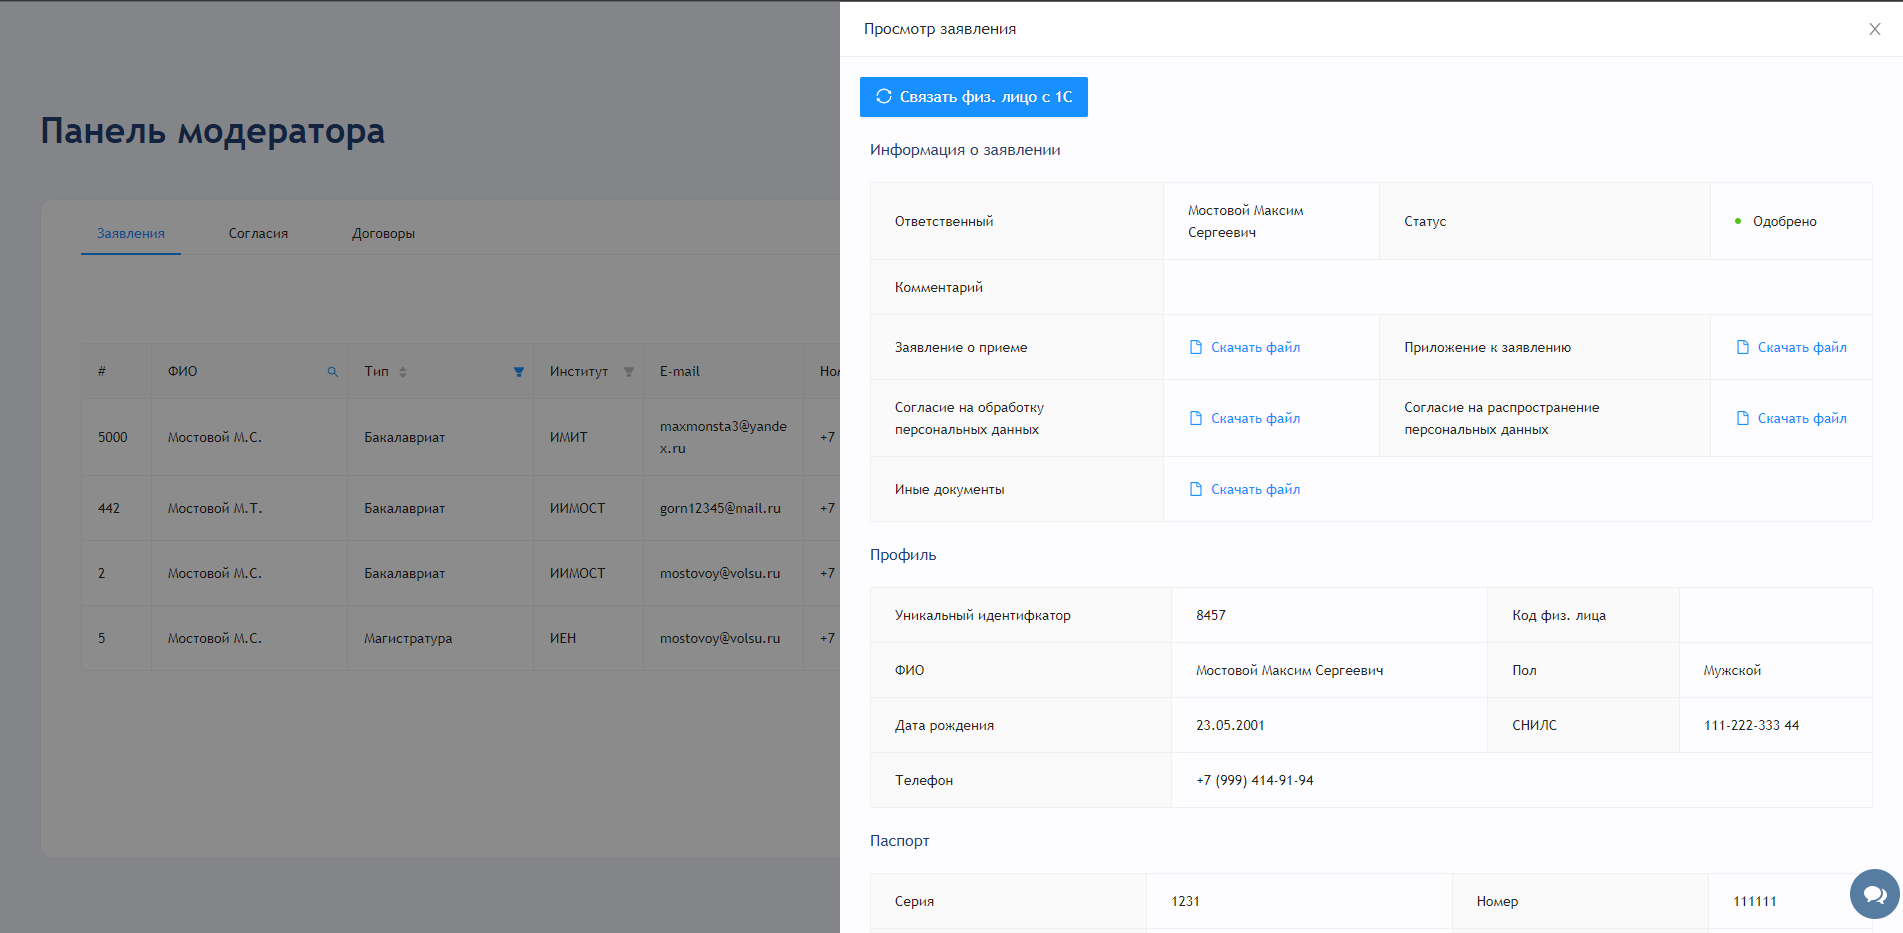
\includegraphics[width=1\hsize]{fig/moderator-view.png}\\[2mm]
\caption{Просмотр полной информации о заявлении на поступление}\label{fig:moderatorstatementview}
\end{center}
\end{figure}

\begin{lstlisting}[caption={Метод добавляющий учетную запись абитуриента в систему учета}, label={ls:moderatoronec}]
const bindUser = () => {
  bindLoading.value = true

  ModerationService.bindUser(props.statement.user_id).then(response => {
    props.statement.user_guid = response.data.result.model
    bindLoading.value = false

    message.success(`Code: ${response.data.result.model})`)
  })
}
\end{lstlisting}

Компоненты просмотра заявления являются общими для просмотра заявления со стороны абитуриента и модератором, обеспечивая таким образом переиспользование написанных компонентов.

Внизу модального окна просмотра заявления находится панель обработки заявления, состояние кнопок обработки заявления меняется в зависимости от статуса заявления (рисунок \ref{fig:moderatorstatementpanel}). Также, сотруднику приемной комиссии доступен список заранее заготовленых причин отклонения заявления (рисунок \ref{fig:moderatorstatenentpanellist}).

\begin{figure}[H]
\begin{center}
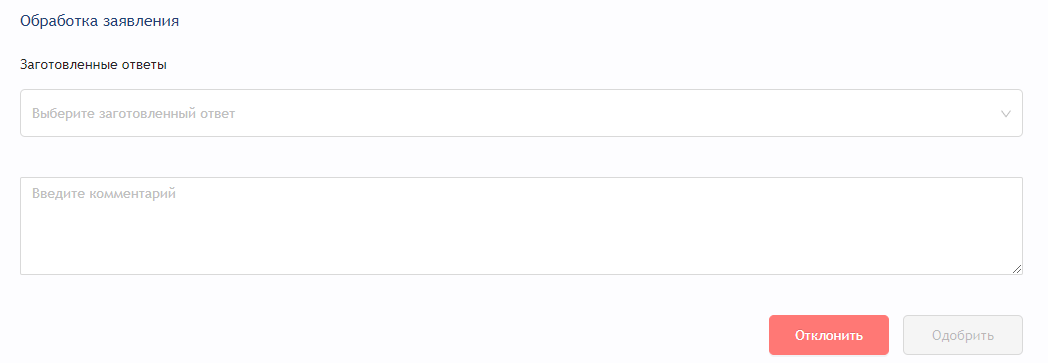
\includegraphics[width=1\hsize]{fig/moderator-statement-panel.png}\\[2mm]
\caption{Панель обработки заявления}\label{fig:moderatorstatementpanel}
\end{center}
\end{figure}

\begin{figure}[H]
\begin{center}
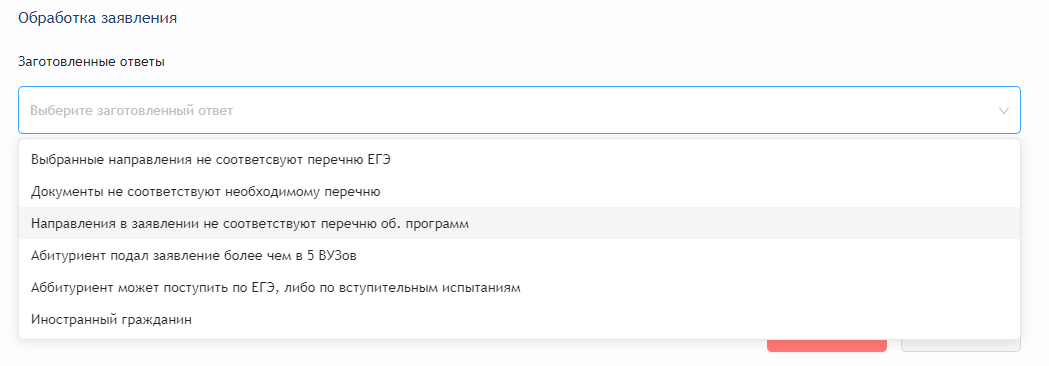
\includegraphics[width=1\hsize]{fig/moderator-statement-cansel-list.png}\\[2mm]
\caption{Список заготовленых причин отклонения заявления}\label{fig:moderatorstatenentpanellist}
\end{center}
\end{figure}

При открытии согласия или заявления, в строке браузера отображается прямая ссылка на открытое согласие или заявление, содержащая его идентификатор, благодаря чему, сотрудник приемной комиссии, может поделится им.

При открытии полной информации об отправленном согласии, сотрудник приемной комиссии может просмотреть всю информацию о согласии, профиль абитуриента, а также открыть заявление на поступление, по которому отправлено согласие (\ref{fig:moderatoragree}). Панель обработки согласия на зачисление аналогична панели обработки заявления на поступление.

\begin{figure}[H]
\begin{center}
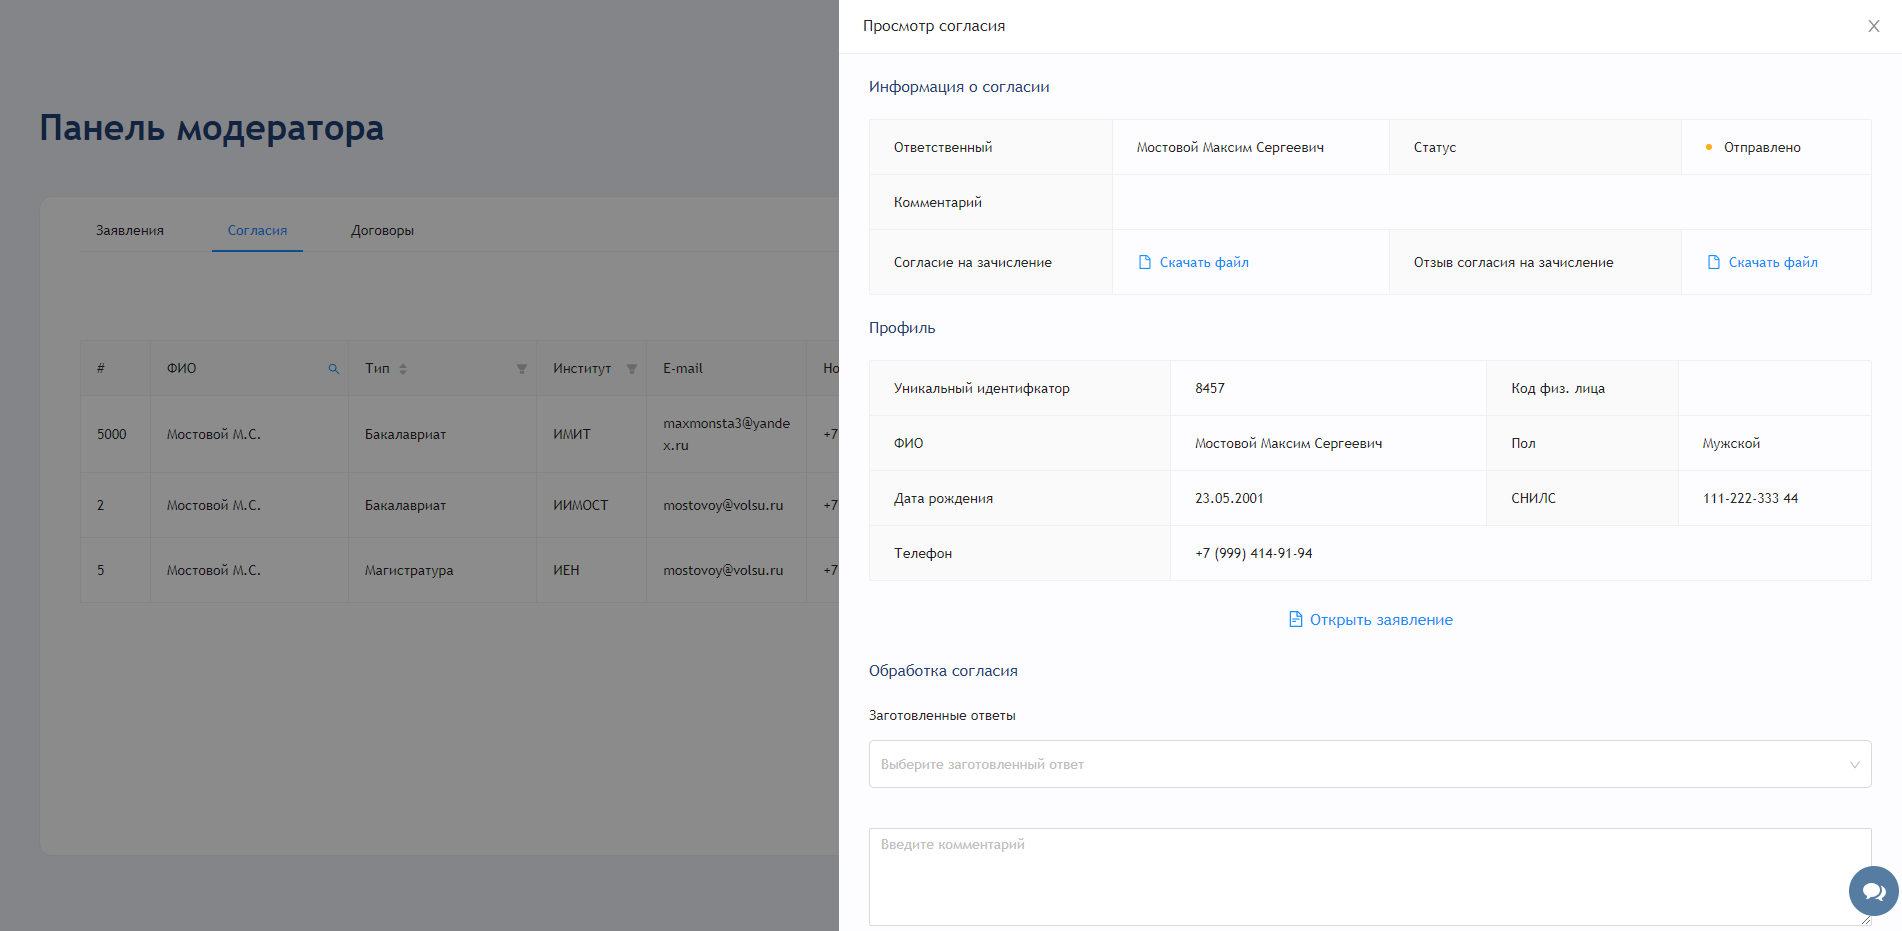
\includegraphics[width=1\hsize]{fig/moderator-agree.png}\\[2mm]
\caption{Просмотр полной информации о согласии на зачисление}\label{fig:moderatoragree}
\end{center}
\end{figure}